% !TEX root = ../AiiDA_tutorial.tex
\maketitle

{\setcounter{tocdepth}{1} \tableofcontents}

\section{Preliminaries}

\ifsshpreparation
%Intro on SSH-ing to Amazon machines
% !TEX root = ../AiiDA_tutorial.tex
%\newpage
\subsection{Instructions to SSH to the Amazon EC2 instance}
\label{sec:sshintro}
You should have received an IP address from the instructors, and two files with a private and a public
SSH key (\verb|aiida_tutorial_NUM| and
\verb|aiida_tutorial_NUM.pub|), where \verb|NUM| is an
integer.
These allow you to connect to an Amazon EC2 instance (different for
each participant of the tutorial). To connect via \texttt{ssh} to this machine follow the steps below, depending on the computer you have.

\textbf{Note!} \emph{If you decide to work in pairs, one of the two people should discard his email. The other person should forward his email to the colleague, and both should then use the same virtual machine IP and account (ssh key). In this case, you will be both using the same account, so be careful not to delete the work of your colleague.}

\subsubsection*{Linux and Mac}	
\begin{itemize}
% \item  If you are using your own laptop, skip this point and go
%   directly to the next one. If your are using one the classroom
%   computer, login into one of the machines using your ETHZ
%   account. If you are not from ETHZ you should have received a
%   username and password to connect first to
%   \texttt{login.phys.ethz.ch} (please do not forget to change this
%   password).
 \item If needed, create a \texttt{.ssh} directory in your home (\verb|mkdir ~/.ssh|), and set its permissions:
   \\ \verb|chmod 700 ~/.ssh|
 \item Copy in this \texttt{.ssh} directory the two files
   \verb|aiida_tutorial_NUM| and\\
   \verb|aiida_tutorial_NUM.pub|
 \item Set the correct permissions on the private key: \\
 \verb|chmod 600 ~/.ssh/aiida_tutorial_NUM| (then check with \verb|ls -l| that the permissions of this file are now \verb|-rw-------|).
 \item Create (or modify if it already exists) the \texttt{config} file in your \texttt{.ssh} directory, adding the following lines:
\begin{verbatim}
Host aiidatutorial
  Hostname IP_ADDRESS
  User aiida
  IdentityFile ~/.ssh/aiida_tutorial_NUM
  LocalForward 8888 localhost:8888
\end{verbatim}
where you have to replace \verb|IP_ADDRESS| with the IP address
provided to you.
 \item You can then \texttt{ssh} to the Amazon EC2 instance from the
   terminal, using simply
 \begin{verbatim}
  ssh -X -C aiidatutorial
 \end{verbatim}
  (connecting with \verb|-X| --- note that sometimes \verb|-Y| is needed
  instead ---
  will allow you to run graphical programs such as xmgrace or
  gnuplot interactively, even if they might not be very responsive as the
  Amazon virtual machines are in Ireland). 
\end{itemize}

\subsubsection*{Windows}
\begin{itemize}
\item Install PuTTY.
\item Run PuTTYGen, load the \verb|aiida_tutorial_NN| private key
  (button \verb|"Load"|). remember to choose to show ``All files
  (*.*)'' in the window, and select the file without any extension
  (Type: File).
\item In the same window, click on ``Save private Key'', and save the
  key with the name\\ \verb|aiida_tutorial_NN.ppk|.
\item Run Pageant: it will add a new icon near the clock, in the
  bottom right of your screen.
\item Right click on this Pageant icon, and click on ``View Keys''.
\item Click on \verb|"Add key"| and select the
  \verb|aiida_tutorial_NN.ppk| you saved a few steps above.
\item Run PuTTY, put the given IP address as hostname. Write \verb|aiidatutorial| in Saved Sessions and click \verb|Save|. Go to Connection $\to$ Data and put \verb|aiida| as autologin username. Under Connection, go to SSH $\to$ Tunnels, type \texttt{8888} in the \texttt{Source Port} box and \texttt{localhost:8888} in \texttt{Destination} and click \verb|Add|.  Click on \verb|Save| again on the Session screen.

\item Now select \verb|aiidatutorial| from the session list, click \verb|Load| and, finally, \verb|open|.

\end{itemize}

\subsection*{Everybody: connect to the machine and start jupyter}

Before starting the tutorial, connect via SSH to the Amazon machine as explained above (the Amazon machine already contains a pre-configured AiiDA installation and some test data for this tutorial).

\fi
% !TEX root = ../AiiDA_tutorial.tex
\subsection*{Before starting}

Once connected to your machine, type in the remote terminal
\begin{bashcommand}
 workon aiida
\end{bashcommand}
This will enable the virtual environment in which AiiDA is installed, allowing you to use AiiDA. %You will need to type this command at every new connection you open to the Amazon machine.

Now type in the same terminal
\begin{bashcommand}
 jupyter notebook --no-browser
\end{bashcommand}
This will run a server with a web application called \texttt{jupyter}, which is used to create interactive python notebooks. To connect to this application, copy the URL that has been printed to the terminal (it will be something like \texttt{http://localhost:8888/?token=2a3ba37cd1...}) and paste it into the URL bar of a web browser. You will see a list of folders: these are folders on the remote Amazon computer.
We will use \texttt{jupyter} in section \ref{sec:querybuilder} and optionally in other sections as well.

Now launch an identical \cmd{ssh} connection (again, as explained above) in another terminal, and type \texttt{workon aiida} here too. This terminal is the one you will actually use in this tutorial.

Note: Since the port listening is set to a specific port (8888) in the section \ref{sec:sshintro}, you have to make sure on the server the Jupiter notebook is running on the port 8888. Otherwise, use an alternative port for listening. 

% \textbf{We suggest to open two terminals with such an \cmd{ssh} connection}:

A final note: for details on AiiDA that may not be fully explained here, you can refer to the full AiiDA documentation, available online at \url{http://aiida-core.readthedocs.io/en/latest/}.

\subsection*{Troubleshooting tips (in case you have issues later)} 
% Should some of these also be in the online version?
\begin{itemize}
\item If you get an error like \texttt{ImportError: No module named aiida} or \texttt{No command 'verdi' found} double check that you have loaded the virtual environment with \texttt{workon aiida} before launching python, ipython or the jupyter server.
\item If your browser cannot connect to the jupyter instance, check that you have correctly configured SSH tunneling/forwarding as described above. Also note that you should run the jupyter server from the terminal connected to the Amazon machine, while the web browser should be opened locally on your laptop or worstation.
\item The Jupyter Notebook officially supports the latest stable versions of Chrome, Safari and Firefox. See \url{http://jupyter-notebook.readthedocs.io/en/4.x/notebook.html#browser-compatibility} for more information on broswer compatibility (and update your browser if it is too old).
% Marco: tested and working on Firefox 53.0.2
% Change this link if we switch to jupyter 5 or later
\end{itemize}




% Day1
% !TEX root = ../AiiDA_tutorial.tex
\section[Verdi command line]{Using the verdi command line}

This part of the tutorial will help to familiarize you with the command-line utility \cmd{verdi}, one of the most common ways to interact with AiiDA. \cmd{verdi} with its subcommands enables a variety of operations such as inspecting the status of ongoing or terminated calculations, showing the details of calculations, computers, codes, or data structures, access the input and the output of a calculation, etc.  Similar to the \texttt{bash} shell, verdi command support Tab completion. Try right now to type \cmd{verdi}, followed by a space, in a terminal and tap Tab twice to have a list of subcommands. Whenever you need the explanation of a command type \cmd{verdi help} or add \cmd{-h} flag if you are using any of the \cmd{verdi} subcommands. 
Finally, fields enclosed in angular brackets, such as \texttt{<pk>}, are placeholders to be replaced by the actual value of that field (an integer, a string, etc...).

\subsection{The list of calculations}
Let us try our first \cmd{verdi} commands. Type in the terminal
\begin{bashcommand}
verdi calculation list
\end{bashcommand}
(Note: the first time you run this command, it might take a few seconds as it is the first time you are accessing the database in the virtual machine. Subsequent calls will be faster).
This will print the list of ongoing calculations, which should be empty. The first output line should look like
\begin{verbatim}
PK    Creation    State    Type    Computer    Job state
----  ----------  -------  ------  ----------  -----------

Total results: 0

Info: last time an entry changed state: never
\end{verbatim}

In order to print a list with all calculations that finished correctly in the AiiDA database, you can use the \cmd{-s/-{}-states} flag as follows:
\begin{bashcommand}
verdi calculation list --states FINISHED
\end{bashcommand}
Another very typical option combination allows to get calculations in \emph{any} state (flag \cmd{-a}) generated in the past \cmd{NUM} days (\cmd{-p <NUM>}): e.g., for calculation in the past 1 day: \cmd{verdi calculation list -p1 -a}. Since you have not yet run any calculations at the virtual machine that you currently use and all the existing calculations were imported and belong to a different user, you can type (flag \cmd{-A} shows the calculations of all the users):
\begin{bashcommand}
verdi calculation list -A --states IMPORTED
\end{bashcommand}

Each row of the output identifies a calculation and shows some information about it. For a more detailed list of properties, choose one row by noting down its PK (primary key) number (first column of the output) and type in the terminal 
\begin{bashcommand}
verdi calculation show <pk>
\end{bashcommand}
The output depends on the specific pk chosen and should inform you about the input nodes (e.g. pseudopotentials, kpoints, initial structure, etc.), and output nodes (e.g. output structure, output parameters, etc.). 

\begin{tcolorbox}
\textbf{PKs/IDs vs.\@ UUIDs}: Beside the (integer) PK, very convenient to reference a calculation or data node
in your database, every node has a UUID (Universally Unique ID) to identify it, that is preserved even when you share some nodes with coworkers---while the PK
will most likely change. You can see the UUID in the output of \texttt{verdi calculation show} or \texttt{verdi node show}. Moreover, if you have already a UUID and you want
to get the corresponding PK in your database, you can use \texttt{verdi node show -u <UUID>},
as we are going to do now.
\end{tcolorbox}

Let us now consider the node with \texttt{UUID = ce81c420-7751-48f6-af8e-eb7c6a30cec3}, which identifies a relaxation of a BaTiO$_3$ unit cell run with Quantum Espresso \cmd{pw.x}.
You can check the information on this node and get the PK with:
\begin{verbatim}
$ verdi node show -u ce81c420-7751-48f6-af8e-eb7c6a30cec3
Property       Value
-------------  ------------------------------------
type           PwCalculation
pk             4235
uuid           ce81c420-7751-48f6-af8e-eb7c6a30cec3
label
description
ctime          2014-10-27 17:51:21.781045+00:00
mtime          2018-05-16 11:19:39.848446+00:00
process state
finish status
computer       [2] daint
code           pw-SVN-piz-daint

Inputs        PK  Type
----------  ----  -------------
parameters  4236  ParameterData
kpoints     4526  KpointsData
pseudo_Ba    966  UpfData
pseudo_Ti   4315  UpfData
settings    4529  ParameterData
pseudo_O    4342  UpfData
structure    436  StructureData

Outputs                    PK  Type
-----------------------  ----  -------------
output_kpoints           3665  KpointsData
output_parameters        3670  ParameterData
output_structure         3666  StructureData
retrieved                3668  FolderData
output_trajectory_array   265  ArrayData
remote_folder            1977  RemoteData
\end{verbatim}
\emph{Keep in mind that you can also use just a part (beginning) of the UUID, as long as it is unique, to show the node information information.} For example, to display the above information, you could also type \cmd{verdi node show -u ce81c420}. In what follows, we are going to mention only the prefixes of the UUIDs since they are sufficient to identify the correct node.

\subsection{A typical AiiDA graph}
\label{sec:aiida_graph}
AiiDA stores inputs required by a calculation as well as the its outputs in the database. These objects are connected in a graph that looks like Fig.~\ref{fig:graph}. We suggest that you have a look to the figure before going ahead.

\begin{figure}
\centering
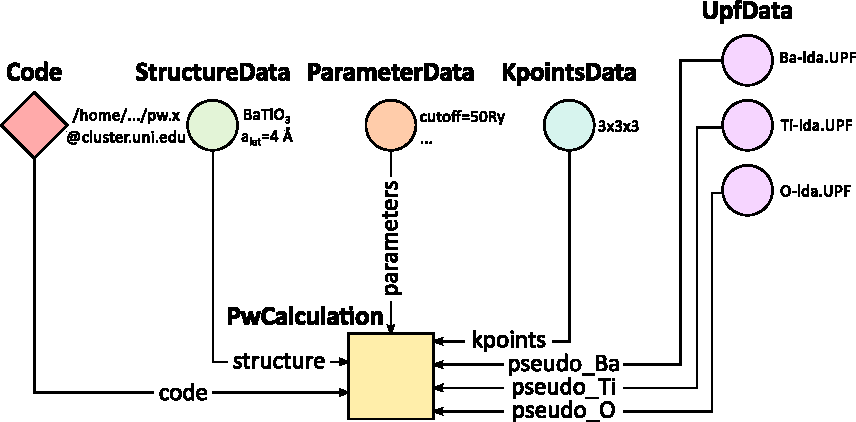
\includegraphics[width=0.5\textwidth]{img/graph/graph-inputonly}

\vspace {1cm}
 
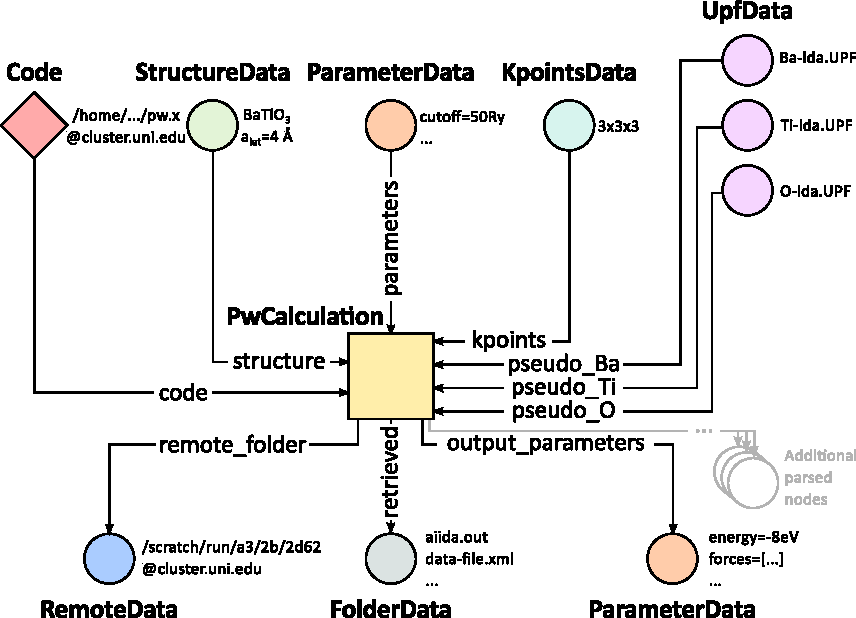
\includegraphics[width=0.5\textwidth]{img/graph/graph-full}
\caption{\label{fig:graph}\textbf{(a, top)} Graph with all inputs (data, circles; and code, diamond) to the Quantum Espresso calculation (square) that you will create in Sec.~\ref{sec:qe} of this tutorial. \textbf{(b, bottom)} Same as (a), but also with the outputs that the daemon will create and connect automatically. The RemoteData node is created during submission and can be thought as a symbolic link to the remote folder in which the calculation runs on the cluster. The other nodes are created when the calculation has finished, after retrieval and parsing. The node with linkname ``retrieved'' contains the raw output files stored in the AiiDA repository; all other nodes are added by the parser. Additional nodes (symbolized in gray) can be added by the parser (e.g., an output StructureData if you performed a relaxation calculation, a TrajectoryData for molecular dynamics, \ldots).}
\end{figure}

You can create a similar graph for any calculation node by using the utility \cmd{verdi graph generate <pk>}. For example, before you obtained information (in text form) for \texttt{UUID = ce81c420}. To visualize similar information in graph(ical) form, run (replacing \cmd{<pk>} with the PK of the node):
\begin{bashcommand}
verdi graph generate <pk>
\end{bashcommand}

This command will create the file \texttt{<pk>.dot} that can be rendered by means of the utility \cmd{dot}. If you now type 
\begin{bashcommand}
dot -Tpdf -o <pk>.pdf <pk>.dot
\end{bashcommand}
you will create a pdf file \texttt{<pk>.pdf}. You can open this file on the Amazon machine by using \cmd{evince} or, if you feel that the ssh connection is too slow, copy it via \cmd{scp} to your local machine.
To do so, if you are using Linux/Mac OS X, you can type in your \emph{local} machine:
\begin{bashcommand}
scp aiidatutorial:<path_with_the_graph_pdf> <local_folder>
\end{bashcommand}
and then open the file. Alternatively, you can use graphical software to achieve the same, for instance: WinSCP on Windows, Cyberduck on the Mac, or the ``Connect to server'' option in the main menu after clicking on the desktop for Ubuntu.

Spend some time to familiarize yourself with the graph structure. Choose the root node (highlighted in blue) and trace back the parent calculation which produced the structure used as an input. This is an example of a Quantum ESPRESSO pw.x calculation, where the input structure was actually obtained as the output of a previous calculation. We will now inspect the different elements of this graph.

\subsection{Inspecting the nodes of a graph}
\subsubsection*{ParameterData and Calculations}
Now, let us have a closer look at the some of the nodes appearing in the graph. 
Choose the node of the type \texttt{ParameterData} with input link name \texttt{parameters}
(to double check, it should have UUID \texttt{d1bbe1ea}) 
and type in the terminal:
\begin{bashcommand}
verdi data parameter show <pk>
\end{bashcommand}
A \texttt{ParameterData} contains a dictionary (i.e., key--value pairs), stored in the database in a format ready to be queried (we will learn how to run queries later on in this tutorial). The command above will print the content dictionary, containing the parameters used to define the input file for the calculation. You can compare the dictionary with the content of the raw input file to Quantum ESPRESSO (that was generated by AiiDA) via the command
\begin{bashcommand}
verdi calculation inputcat <pk>
\end{bashcommand}
where you substitute the pk of the calculation node. 
Check the consistency of the parameters written in the input file and those stored in the ParameterData node. Even if you don't know the meaning of the input flags of a Quantum ESPRESSO calculation, you should be able to see how the input dictionary
has been converted to Fortran namelists. 

The previous command just printed the content of the ``default'' input file \texttt{aiida.in}. 
To see a list of all the files used to run a calculation (input file, submission script, etc.) instead type
\begin{bashcommand}
verdi calculation inputls <pk>
\end{bashcommand}
(Adding a \texttt{-{}-color} flag allows you to easily distinguish files from folders by a different coloring).

Once you know the name of the file you want to visualize, you can call the \cmd{verdi 
calculation inputcat} command specifying the path. For instance, to see the submission
script, you can do:
\begin{bashcommand}
verdi calculation inputcat <pk> -p _aiidasubmit.sh
\end{bashcommand}

%%%%%%%%%%%%%%%%%%%%%%Structure data%%%%%%%%%%%%%%%%%%%
\subsubsection*{StructureData}
Now let us focus on StructureData objects, representing a crystal structure.
We can consider for instance the input structure to the calculation we were 
considering before (it should have UUID prefix \texttt{3a4b1270}).
Such objects can be inspected interactively by means of an atomic viewer such as the one provided by \texttt{ase}. AiiDA however supports several other viewers such as \texttt{xcrysden}, \texttt{jmol}, and \texttt{vmd}. Type in the terminal 
\begin{bashcommand}
verdi data structure show --format ase <pk>
\end{bashcommand}
to show the selected structure (it will take a few seconds to appear, and you can rotate the view with the right mouse button---if
you receive some errors, make sure you started your SSH connection with the 
\texttt{-X} or \texttt{-Y} flag).

Alternatively, especially if showing them interactively is too slow over SSH, you can export the content of a structure node in various popular formats such as \texttt{xyz} or \texttt{xsf}. This is achieved by typing in the terminal
\begin{bashcommand}
verdi data structure export --format xsf <pk>  >  <pk>.xsf
\end{bashcommand}
You can open the generated \texttt{xsf} file and observe the cell and the coordinates. Then, you can then copy \texttt{<pk>.xsf} from the Amazon machine to your local one and then visualize it, e.g. with xcrysden (if you have it installed):
\begin{bashcommand}
xcrysden --xsf <pk>.xsf
\end{bashcommand}

%%%%%%%%Verdi code%%%%%%%%%%%%
\subsubsection*{Codes and computers}
Let us focus now on the nodes of type \texttt{code}. A code represents (in the database) the actual executable used to run the calculation. Find the pk of such a node in the graph and type
\begin{bashcommand}
verdi code show <pk>
\end{bashcommand}

The command prints information on the plugin used to interface the code to AiiDA, the remote machine on which the code is executed, the path of its executable, etc. To show a list of all available codes type
\begin{bashcommand}
verdi code list
\end{bashcommand}
If you want to show all codes, including hidden ones and those created by other users, use \texttt{verdi code list -a -A}. Now, among the entries of the output you should also find the code just shown.

%%%%%%%%%%%Verdi computer%%%%%%%%%%
Similarly, the list of computers on which AiiDA can submit calculations is accessible by means of the command
\begin{bashcommand}
verdi computer list -a
\end{bashcommand}
(\cmd{-a} shows all computers, also the one imported in your database but that you did not configure, i.e., to which you don't have access).
Details about each computer can be obtained by the command 
\begin{bashcommand}
verdi computer show <COMPUTERNAME>
\end{bashcommand}
Now you have the tools to answer the question:
\begin{tcolorbox}
What is the scheduler installed on the computer where the calculations of the graph have run?
\end{tcolorbox}


%%%%%%%%%%%%%%%verdi output|res%%%%%%%%%%%%%%%%
\subsubsection*{Calculation results}
The results of a calculation can be accessed directly from the calculation node. Type in the terminal
\begin{bashcommand}
verdi calculation res <pk>
\end{bashcommand}
which will print the output dictionary of the ``scalar'' results parsed by AiiDA at the end of the calculation.  Note that this is actually a shortcut for 
\begin{bashcommand}
verdi data parameter show <pk2>
\end{bashcommand}
where \texttt{pk2} refers to the ParameterData node attached as an output of the calculation node, with link name \texttt{output\_parameters}.

\begin{tcolorbox}
By looking at the output of the command, what is the Fermi energy of the calculation with UUID prefix \texttt{ce81c420}?
\end{tcolorbox}



%%%%%%%%%%%%verdi output cat%%%%%%%%%%%
Similarly to what you did for the calculation inputs, you can access the output files via the commands
\begin{bashcommand}
verdi calculation outputls <pk>
\end{bashcommand}
and
\begin{bashcommand}
verdi calculation outputcat <pk>
\end{bashcommand}
Use the latter to verify that the Fermi energy that you have found in the last step has been extracted correctly from the output file (Hint: filter the lines containing the string ``Fermi'', e.g. using \texttt{grep}, to isolate the relevant lines). 

%%%%%%%%%%%verdi data array show%%%%%%%%%%%%
The results of calculations are stored in two ways: \texttt{ParameterData} objects are stored in the database, which makes querying them very convenient, whereas \texttt{ArrayData} objects are stored on the disk. Once more, use the command \cmd{verdi data array show <pk>} to know the Fermi energy obtained from calculation with UUID prefix \texttt{ce81c420} (you need to use, this time, the PK of the output ArrayData of the calculation, with link name \cmd{output\_trajectory\_array}). As you might have realized the difference now is that the whole series of values of the Fermi energy calculated after each relax/vc-relax step are stored. (The choice of what to store in \texttt{ParameterData} and \texttt{ArrayData} nodes is made by the parser of \texttt{pw.x} implemented in the \texttt{aiida-quantumespresso} plugin.)

%%%%%%%%%%%verdi comments%%%%%%%%%%%%%%5
\subsubsection*{(Optional section) Comments}
AiiDA offers the possibility to attach comments to a calculation node, in order to be able to remember more easily its details. Node with UUID prefix ce81c420 has no comment already defined, but you can add a very instructive one by typing in the terminal
%%%%%%%%%%verdi comment%%%%%%%%%%%%%%
\begin{bashcommand}
verdi comment add -c "vc-relax of a BaTiO3 done with QE pw.x" <pk>
\end{bashcommand}
Now, if you ask for a list of all comments associated to that calculation by typing
\begin{bashcommand}
verdi comment show <pk>
\end{bashcommand}
the comment that you just added will appear together with some useful information such as its creator and creation date. We let you play with the other options of \cmd{verdi comment} command to learn how to update or remove comments.


% %%%%%%%%%%TO BE DISCUSSED%%%%%%%%%%%%%%%%%%
% \textcolor{red}{We might discuss the \cmd{verdi node repo ls|cat command} e.g.}
% \begin{bashcommand}
% verdi node repo cat -p 4079 raw_input/aiida.in 
% \end{bashcommand}
% \textcolor{red}{Moreover, at this state no RemoteData concept has been introduced}


\subsection{AiiDA groups of calculations}
In AiiDA, calculations (and more generally nodes) can be organized in groups, which are particularly useful to assign a set of calculations or data to a common project. This allows you to have quick access to a whole set of calculations with no need for tedious browsing of the database or writing complex scripts for retrieving the desired nodes. Type in the terminal
\begin{bashcommand}
verdi group list
\end{bashcommand}
to show a list of the groups that already exist in the database. Choose the PK of the group named \texttt{tutorial\_pbesol} and look at the calculations that it contains by typing
\begin{bashcommand}
verdi group show <pk>
\end{bashcommand}
In this case, we have used the name of the group to organize calculations according to the pseudopotential that has been used to perform them. Among the rows printed by the last command you will be able to find the calculation we have been inspecting until now. 

If, instead, you want to know all the groups to which a specific node belomngs, you can run 
\begin{bashcommand}
verdi group list --node <pk> 
\end{bashcommand}


% !TEX root = ../AiiDA_tutorial.tex
\section[Verdi shell and AiiDA objects]{Using the verdi shell and familiarizing
with AiiDA objects\label{shell}}

In this section we will use an interactive ipython environment with all the basic AiiDA classes
already loaded. We propose two realizations of such a tool. The first consist of a special ipython shell where all the AiiDA classes, methods and functions are accessible.
Type in the terminal
%Open a second terminal, connect to the Amazon machine with \cmd{ssh} and type: 
\begin{bashcommand}
 verdi shell
\end{bashcommand}
For all the everyday AiiDA-based operations, i.e. creating,
querying and using AiiDA objects, the \cmd{verdi shell} is probably the best tool.
In this case, we suggest that you use two terminals, one for the \cmd{verdi shell} and one to execute bash commands.

The second option is based on \texttt{jupyter} notebooks and is probably most suitable to the purposes of our tutorial. Go to the browser where you have opened \texttt{jupyter} and click \texttt{New} $\to$ \texttt{Python 2} (top right corner). This will open an ipython notebook based on cells where you can type portions of python code. The code will not be executed until you press \verb|Shift+Enter| from within a cell. 
Type in the first cell 
\begin{pythoncommand}
 %aiida
\end{pythoncommand}
and execute it. This will set exactly the same environment as the \cmd{verdi shell}.
The notebook will be automatically saved upon any modification and when you think you are done, you can export your notebook in many formats by going to \verb|File| $\to$ \verb|Download as|. We suggest you to have a look to the drop-down menus \texttt{Insert} and \texttt{Cell} where you will find the main commands to manage the cells of your notebook. 
\textbf{The \cmd{verdi shell} and the \cmd{jupyter} notebook are completely equivalent. Use either according to your personal preference.}

Note: you will still need sometimes to type command-line
instructions in \cmd{bash} in the first terminal you opened today. 
To differentiate these from the commands to be typed in the
\cmd{verdi shell}, the latter will be marked in this document by a vertical line
on the left, like:
\begin{pythoncommand}
 some verdi shell command
\end{pythoncommand}
while command-line instructions in \cmd{bash} to be typed on a terminal will
be encapsulated between horizontal lines:
\begin{bashcommand}
 some bash command
\end{bashcommand}
Alternatively, to avoid changing terminal, you can execute \cmd{bash} commands within the \cmd{verdi shell} or the notebook adding an exclamation mark before the command itself
\begin{pythoncommand}
 !some bash command
\end{pythoncommand}


%%%%%%%%%%%%%%%%%%%%%%%%%%%%%%%
% Load node and .res method
%%%%%%%%%%%%%%%%%%%%%%%%%%%%%%%

\subsection[load_node]{Loading a node\label{load_node}}

Most AiiDA objects are represented by nodes, identified in the database by its pk number (an integer). 
You can access a node using the following command in the shell:
\begin{pythoncommand}
 node = load_node(PK)
\end{pythoncommand}
Load a node using one of the calculation pks visible in the graph you displayed
in the previous section of the tutorial. Then get the energy of the
calculation with the command
\begin{pythoncommand}
 node.res.energy
\end{pythoncommand}
You can also type
\begin{pythoncommand}
 node.res.
\end{pythoncommand}
and then press \cmd{TAB} to see all the possible output
results of the calculation.

%%%%%%%%%%%%%%%%%%%%%%%%%%%%%%%
% Loading several kinds of nodes
%%%%%%%%%%%%%%%%%%%%%%%%%%%%%%%

\subsection{Loading different kinds of nodes}

\subsubsection{Pseudopotentials}

From the graph displayed in Section~\ref{sec:aiida_graph}, find the pk of the barium pseudopotential file (LDA). Load it and verify that it describes barium. Type
\begin{pythoncommand}
 upf = load_node(PK)
 upf.element
\end{pythoncommand}
All methods of \texttt{UpfData} are accessible by typing \texttt{upf.} and then pressing \cmd{TAB}.

\subsubsection{k-points}

A set of k-points in the Brillouin zone is represented by an instance of the
\texttt{KpointsData} class. Choose one from the graph of Section~\ref{sec:aiida_graph},
load it as \texttt{kpoints} and inspect its content:
% kpoints = load_node(PK)
\begin{pythoncommand}
 kpoints.get_kpoints_mesh()
\end{pythoncommand}
Then get the full (explicit) list of k-points belonging to this mesh using
\begin{pythoncommand}
 kpoints.get_kpoints_mesh(print_list=True)
\end{pythoncommand}
If you incurred in a \texttt{AttributeError}, it means that the kpoints instance does not 
represent a regular mesh but rather a list of 
k-points defined by their crystal coordinates (typically used when plotting a band structure).
In this case, get the list of k-points coordinates using
\begin{pythoncommand}
 kpoints.get_kpoints()
\end{pythoncommand}
If you prefer Cartesian (rather than crystal) coordinates, type
\begin{pythoncommand}
 kpoints.get_kpoints(cartesian=True)
\end{pythoncommand}

%%%%%%%%%K points%%%%%%%%%%5
%\subsubsection{K-points definition}
For later use in this tutorial, let us try now to create a kpoints instance, to 
describe a regular $2\times2\times2$ mesh of k-points, centered at the Gamma point (i.e. without offset).
This can be done with the following commands:
\begin{pythoncommand}
 from aiida.orm.data.array.kpoints import KpointsData
 kpoints = KpointsData()
 kpoints_mesh = 2
 kpoints.set_kpoints_mesh([kpoints_mesh,kpoints_mesh,kpoints_mesh])
 kpoints.store()
\end{pythoncommand}

The import performed in the first line is however unpractical as it requires to remember the exact location of the module containing the KpointsData class. Instead, it is easier to use the \cmd{DataFactory} function instead of an explicit import.

\begin{pythoncommand}
 KpointsData = DataFactory("array.kpoints")
\end{pythoncommand}

This function loads the appropriate class defined in a string (here \texttt{array.kpoints}).\footnote{The string provided to the \cmd{DataFactory} encodes both the location and the name of the required class according to some specific rules.}
Therefore, \texttt{KpointsData} is not a class instance, but the kpoints class itself!


\subsubsection{Parameters}

Nested dictionaries with individual parameters, as well as lists and arrays, are
represented in AiiDA with \texttt{Parameter\-Data} objects. Get the PK and load
the input parameters of a calculation in the graph of Section~\ref{sec:aiida_graph}.
Then display its content by typing
\begin{pythoncommand}
 params.get_dict()
\end{pythoncommand}
where \texttt{params} is the \texttt{ParameterData} node you loaded. %You can
%also access directly the first level of dictionary keys by pressing \cmd{TAB}
%after having typed
%\begin{pythoncommand}
% params.dict.
%\end{pythoncommand}
Modify the dictionary content so that the wave-function cutoff is now set to 20 Ry. 
Note that you cannot modify an object already stored in the database.
To save the modification, you must create a new ParameterData object. Similarly to what discussed before, first load the \texttt{ParameterData} class by typing
\begin{pythoncommand}
 ParameterData = DataFactory('parameter')
\end{pythoncommand}
Then an instance of the class (i.e. the parameter object
that we want to create) is created and initialized by the command
\begin{pythoncommand}
 new_params = ParameterData(dict=YOUR_DICT)
\end{pythoncommand}
where \texttt{YOUR\_DICT} is the modified dictionary.
Note that the parameter object is not yet stored in the database.
In fact, if you simply type \texttt{new\_params} in the verdi shell, you will be prompted with a string notifying you the ``unstored'' status.
To save an entry in the database corresponding to the \texttt{new\_params} object, you need to type a last command in the verdi shell:
\begin{pythoncommand}
 new_params.store()
\end{pythoncommand}

\subsubsection{Structures}

Find a structure in the graph of Section~\ref{sec:aiida_graph} and load it. Display
its chemical formula, atomic positions and species using
\begin{pythoncommand}
 structure.get_formula()
 structure.sites
\end{pythoncommand}
where \texttt{structure} is the structure you loaded. If you are familiar with ASE and PYMATGEN,
you can convert this structure to those formats by typing
\begin{pythoncommand}
 structure.get_ase()
 structure.get_pymatgen()
\end{pythoncommand}
%You then have access to all the ASE/PYMATGEN methods.
Let's try now to define a new structure to study, specifically a silicon
crystal.
In the \cmd{verdi shell}, define a cubic unit cell as a $3\times3$ matrix, with lattice parameter $a_{lat}=5.4$ \AA:
\begin{pythoncommand}
 alat = 5.4
 the_cell = [[alat/2,alat/2,0.],[alat/2,0.,alat/2],[0.,alat/2,alat/2]]
\end{pythoncommand}

{\bf Note}: Default units for crystal structure cell and coordinates in AiiDA are \AA.

Structures in AiiDA are instances of \texttt{StructureData} class: load it in the verdi shell
\begin{pythoncommand}
 StructureData = DataFactory("structure")
\end{pythoncommand}
Now, initialize the class instance (i.e.\ is the structure we want to study) by the command
\begin{pythoncommand}
 structure = StructureData(cell=the_cell)
\end{pythoncommand}
which sets the cubic cell defined before. From now on, you can access the cell with the command
\begin{pythoncommand}
 structure.cell
\end{pythoncommand}
Finally, append each of the 2 atoms of the cell command. You can do it
using commands like
\begin{pythoncommand}
 structure.append_atom(position=(alat/4.,alat/4.,alat/4.),symbols="Si")
\end{pythoncommand}
for the first `Si' atom. Repeat it for the other atomic site $\left(0,0,0\right)$.
You can access and inspect\footnote{if you set the structure incorrectly, for example with overlapping atoms, it is very likely that any DFT code will fail!} the structure sites with the command
\begin{pythoncommand}
 structure.sites
\end{pythoncommand}
If you make a mistake, start over from \texttt{structure = StructureData(cell=the\_cell)}, or equivalently use \\
\texttt{structure.clear\_kinds()} to remove all kinds (atomic species) and sites.
Alternatively, AiiDA structures can also be
converted directly from ASE~\cite{ref:ASE} structures using\footnote{We purposefully do not provide advanced commands
for crystal structure manipulation in AiiDA, because python packages that accomplish such tasks
already exist (such as ASE or pymatgen).}
\begin{pythoncommand}	
 from ase.lattice.spacegroup import crystal
 ase_structure = crystal('Si', [(0,0,0)], spacegroup=227,
                 cellpar=[alat, alat, alat, 90, 90, 90],primitive_cell=True)
 structure=StructureData(ase=ase_structure)
\end{pythoncommand}
%
Now you can store the new structure object in the database with the command:
\begin{pythoncommand}
 structure.store()
\end{pythoncommand}
%
%
Finally, we can also import the silicon structure from an external (online) repository
such as the Crystallography Open Database~\cite{ref:COD}:
\begin{pythoncommand}
from aiida.tools.dbimporters.plugins.cod import CodDbImporter 
importer = CodDbImporter()
for entry in importer.query(formula='Si',spacegroup='F d -3 m'):
        structure = entry.get_aiida_structure()
        print "Formula", structure.get_formula()
        print "Unit cell volume: ", structure.get_cell_volume()
\end{pythoncommand}
In that case two duplicate structures are found for Si.
%\footnote{Note: one could compare these two structures with the pymatgen tool
%StructureMatcher}

%%%%%%%%%%%%%%%%%%%%%%%%%%%%%%%
% .inp / .out methods
%%%%%%%%%%%%%%%%%%%%%%%%%%%%%%%

\subsection{Accessing inputs and outputs}

Load again the calculation node used in Section~\ref{load_node}:
\begin{pythoncommand}
 calc = load_node(PK)
\end{pythoncommand}
Then type
\begin{pythoncommand}
 calc.inp.
\end{pythoncommand}
and press \cmd{TAB}: you will see all the link names between the
calculation and its input nodes. You can use a specific linkname to access the
corresponding input node, e.g.:
\begin{pythoncommand}
 calc.inp.structure
\end{pythoncommand}

You can use the \cmd{inp} method multiple times in order to browse the graph. For instance, 
if the input structure node that you just accessed is the output of another calculation, you can access the latter by typing

\begin{pythoncommand}
 calc2 = calc.inp.structure.inp.output_structure
\end{pythoncommand}
Here \texttt{calc2} is the \texttt{PwCalculation} that produced the structure used as an input for \texttt{calc}.

Similarly, if you type:
\begin{pythoncommand}
 calc2.out.
\end{pythoncommand}
and then \cmd{TAB}, you will list all output link names of the calculation.
One of them leads to the structure that was the input of \texttt{calc} we loaded
previously:
\begin{pythoncommand}
 calc2.out.output_structure
\end{pythoncommand}
Note that links have a single name, that was assigned by the
calculation that used the corresponding input or produced the corresponding
output, as illustrated in Fig.~\ref{fig:graph}.

For a more programmatic approach, you can get a list of the inputs and outputs of a node, say \texttt{calc}, with the methods
\begin{pythoncommand}
 calc.get_inputs()
 calc.get_outputs()
\end{pythoncommand}

Alternatively, you can get a dictionary where the keys are the link names and the values are the linked objects, with the methods
\begin{pythoncommand}
 calc.get_inputs_dict()
 calc.get_outputs_dict()
\end{pythoncommand}

Note: You will sometime see entries in the dictionary with names like \texttt{output\_kpoints\_3511}.  These exist because standard python dictionaries require unique key names while link labels may not be unique. Therefore, we use the link label plus the PK separated by underscores.


%%%%%%%%%%%%%%%%%%%%%%%%%%%%%%%%%%%%%
% Upf Families
%%%%%%%%%%%%%%%%%%%%%%%%%%%%%%%%%%%%%

\subsection{Pseudopotential families}

Pseudopotentials in AiiDA are grouped in ``families'' that contain one
single pseudo per element. We will see how to work with UPF pseudopotentials (the format used by Quantum ESPRESSO and some other codes).\\
Download and untar the SSSP~\cite{ref:SSSP} pseudopotentials via the
commands:
% wget http://www.materialscloud.org/sssp/pseudos/SSSP_eff_PBESOL.tar.gz
\begin{bashcommand}
 wget https://archive.materialscloud.org/file/2018.0001/v1/SSSP_efficiency_pseudos.tar.gz
 tar -zxvf SSSP_efficiency_pseudos.tar.gz
\end{bashcommand}
Then you can upload the whole set of pseudopotentials to AiiDA by to the following
\texttt{verdi} command:
\begin{bashcommand}
verdi data upf uploadfamily SSSP_efficiency_pseudos 'SSSP' 'SSSP pseudopotential library'
\end{bashcommand}
In the command above, \texttt{SSSP\_efficiency\_pseudos} is the folder containing the pseudopotentials, 'SSSP' is the name given to the family and the last
argument is its description.\\
Finally, you can list all the pseudo families present in the database with
\begin{bashcommand}
 verdi data upf listfamilies
\end{bashcommand}


% !TEX root = ../AiiDA_tutorial.tex
%%%%%%%%%INTRO%%%%%%%%%
\section[Submit, monitor and debug calculations]{\label{sec:qe}Submit, monitor and debug calculations}
The goal of this section is to understand how to create new data in AiiDA. We will launch a total energy calculation and check its results. We will introduce intentionally some common mistakes along the process of defining and submitting a calculation and we will explain you how to recognize and correct them. While this debugging is done here `manually', workflows  (that we will learn later in this tutorial) can automate this procedure considerably. 
%Optionally, you will run a band structure calculation using a previous (``parent'') calculation.
For computing the DFT energy of the silicon crystal (with a PBE functional) we will use Quantum ESPRESSO~\cite{ref:QE}, in particular the PWscf code (\texttt{pw.x}).
Besides the AiiDA-core package, a number of plugins exist for many different codes.
These are listed in the \href{https://aiidateam.github.io/aiida-registry/}{AiiDA plugin registry}\footnote{\url{https://aiidateam.github.io/aiida-registry/}}.
In particular, the ``aiida-quantumespresso'' plugin (already installed in your machine) provides a very extensive set of plugins, covering most (if not all) the functionalities of the underlying codes.


\subsection{The AiiDA daemon}

First of all, check that the AiiDA daemon is actually running. The AiiDA daemon is a program running all the time in the background, checking if new calculations appear and need to be submitted to the scheduler\footnote[1]{i.e. first queued on the cluster, and then run when the queuing system allows it}. The daemon also takes care of all the necessary operations before the calculation submission\footnote[2]{creating a directory where to run and copying there the input files}, and after the calculation has completed on the cluster.\footnote[3]{retrieving and copying some of the output files in the database repository, parsing one or several output files, attaching some data to the calculation and storing them in the database.}
Type in the terminal
\begin{bashcommand}
verdi daemon status
\end{bashcommand}
If the daemon is running, the output should look like

\begin{verbatim}
    Profile: default
    Daemon is running as PID 1650 since 2018-05-16 16:26:04
    Active workers [1]:
      PID    MEM %    CPU %  started
    -----  -------  -------  -------------------
     1653    8.225        0  2018-05-16 16:26:04
    Use verdi daemon [incr | decr] [num] to increase / decrease the amount of workers
\end{verbatim}
If this is not the case, type in the terminal
\begin{bashcommand}
verdi daemon start
\end{bashcommand}
to start the daemon.


%%%%%%%%%%%%%%CREATE AND SUBMIT CALCULATION%%%%%%%%%%%%%
%N.B. In the old tutorial calculation are submitted via the interactive shell, whereas here users will do it via verdi run <script_name>
%%%%%%%%%%%%%%%
\subsection{Creating a new calculation\label{sec:create_calc}}
To launch a calculation, you will need to interact with AiiDA mainly in the \cmd{verdi shell}.
We strongly suggest you to first try the commands in the shell, and then copy them in a script ``test\_pw.py'' using a text editor. This will be very useful for later execution of a similar series of commands.

\textbf{The best way to run python scripts using AiiDA functionalities is to run them in a terminal by means of the command}
\begin{bashcommand}
 verdi run <scriptname>
\end{bashcommand}

Every calculation sent to a cluster is linked to a code, which describes the executable file to be used.
Therefore, first load the suitable code:
\begin{pythoncommand}
 code = Code.get_from_string(<codename>)
\end{pythoncommand}
Here \texttt{Code} is the general AiiDA class handling all possible codes, and \texttt{code} is a class instance tagged as \texttt{<codename>} (see the first part of the tutorial for listing all codes installed in your AiiDA machine).
You might also want to list only the codes that define a default calculation plugin for the pw.x code of Quantum ESPRESSO. You can do this with the following command:
\begin{bashcommand}
verdi code list -p quantumespresso.pw
\end{bashcommand}
Pick the correct codename, that might look like, e.g. \texttt{qe-pw-6.2.1@localhost}.

Once run, AiiDA calculations are instances of the class \texttt{Calculation}, more precisely of one of its subclasses, each corresponding to a code specific plugin (for example, the PWscf plugin). You have already seen \texttt{Calculation} classes in the previous sections.

However, to create a new calculation, rather than manually creating a new class, 
the suggested way is to use a \texttt{Builder}, that helps in setting the various
calculation inputs and parameters, and provides TAB-completion.

To obtain a new builder, we can use the \texttt{get\_builder} method of the \texttt{code} object:
\begin{pythoncommand}
 builder = code.get_builder()
\end{pythoncommand}
This returns a builder that helps in setting up the inputs for the \texttt{PwCalculation} class (associated to the \texttt{quantumespresso.pw} plugin, i.e. the default 
plugin for the code you chose before).

As the first step, you can assign a (short) label or a (long) description
to the calculation that you are going to create, that you might find 
convenient in the future. This can be achieved with:
\begin{pythoncommand}
 builder.label = "PW test"
 builder.description = "My first AiiDA calc with Quantum ESPRESSO on BaTiO3"
\end{pythoncommand}
This information will be saved in the database for later query or inspection.
Note that you can press TAB after writing \texttt{builder.} to see all available inputs.

Now you have to specify the number of machines (a.k.a. cluster nodes) you are going to run on and the maximum time allowed for the calculation. These general calculation options,
that are independent of the code or plugin, but rather mainly passed later to the scheduler
that handles the queue, are all grouped under ``builder.options'':
\begin{pythoncommand}
 builder.options.resources = {'num_machines': 1}
 builder.options.max_wallclock_seconds = 30*60
\end{pythoncommand}
Just like the normal inputs, these builder options are also TAB-completed.
Type "builder.options." and hit the TAB button to see the list of available options.

%%%%%%%%%%%%%%%%%%%%%%
\subsubsection{Preparation of inputs}
Quantum ESPRESSO requires an input file containing Fortran namelists and variables, plus some cards sections (the documentation is available \href{http://www.quantum-espresso.org/wp-content/uploads/Doc/INPUT_PW.html}{online}\footnote{\url{http://www.quantum-espresso.org/wp-content/uploads/Doc/INPUT_PW.html}}).
The Quantum ESPRESSO plugin of AiiDA requires quite a few nodes in input, which are documented 
\href{http://aiida-core.readthedocs.io/en/latest/plugins/quantumespresso/pw.html}{online}\footnote{\url{http://aiida-core.readthedocs.io/en/latest/plugins/quantumespresso/pw.html}}.
Here we will instruct our calculation with a minimal configuration for computing the energy of silicon. We need:
\begin{enumerate}
\item Pseudopotentials
\item a structure
\item the k-points
\item the input parameters
\end{enumerate}
We leave the parameters as the last thing to setup and start with structure, k-points, and pseudopotentials.

\begin{tcolorbox}
Use what you learned in the previous section and define these two kinds of objects in this script.
Define in particular a silicon structure and a 2$\times$2$\times$2 mesh of k-points.
Notice that if you just copy and paste the code that you executed previously, you will create duplicated information in the database (i.e. every time you will execute the script, you will create another StructureData, another KpointsData, \dots).
In fact, you already have the opportunity to re-use an already existing structure.\footnote{However, to avoid duplication of KpointsData, you should first learn how to query the database, therefore we will ignore this duplication issue for now.}
Use therefore a combination of the bash command \cmd{verdi data structure list} and of the shell command \texttt{load\_node()} to get an object representing the structure created earlier.
%For the KpointsData instead we will ignore this duplication for the time being, and you can simply use the same code of this morning.
\end{tcolorbox}

\subsubsection{Attaching the input information to the calculation}
So far we have defined (or loaded) some of the input data, but we haven't instructed the calculation to use them.
To do this, let's just set the appropriate attributes of the builder (we assume here 
that you created the structure and k-points AiiDA nodes before and called them 
\texttt{structure} and \texttt{kpoints}, respectively):
\begin{pythoncommand}
 builder.structure = structure
 builder.kpoints = kpoints
\end{pythoncommand}
Note that you can set in the builder both stored and unstored nodes.
AiiDA will take care of storing the unstored nodes upon submission. Otherwise,
if you decide not to submit, nothing will be stored in the database.

Moreover, PWscf also needs information on the pseudopotentials, specified by UpfData objects.
This is set by storing a dictionary in ``builder.pseudo'', with keys being the
kind names, and value being the UpfData pseudopotential nodes.
To simplify the task of choosing pseudopotentials, we can however use a helper
function that automatically returns this dictionary picking the pseudopotentials
from a given UPF family.

You can list the preconfigured families from the command line:
\begin{bashcommand}
 verdi data upf listfamilies
\end{bashcommand}
Pick the one you configured earlier or one of the \texttt{SSSP} families that we provide, and link it to the calculation using the command:
\begin{pythoncommand}
 from aiida.orm.data.upf import get_pseudos_from_structure
 builder.pseudo = get_pseudos_from_structure(structure, '<PSEUDO_FAMILY_NAME>')
\end{pythoncommand}



\subsubsection{Preparing and debugging input parameters}
The last thing we miss is a set of parameters (i.e. cutoffs, convergence thresholds, etc\dots) to launch the Quantum ESPRESSO calculation.
This part requires acquaintance with Quantum ESPRESSO and, very often, this is the part to tune when a calculation shows a problem.
Let's therefore use this part of the tutorial to learn how to debug problems, and {\bf let's introduce errors intentionally}.
Note also that some of the problems we will investigate appear the first times you launch calculations and can be systematically avoided by using workflows.


Let's define a set of input parameters for Quantum ESPRESSO, preparing a dictionary of the form:
\begin{pythoncommand}
parameters_dict = {
    'CONTROL': {
        'calculation': 'scf',
        'tstress': True,
        'tprnfor': True,
    },
    'SYSTEM': {
        'ecutwfc': 30.,
        'ecutrho': 200.,
        'mickeymouse': 240.,
    },
    'ELECTRONS': {
        'conv_thr': 1.e-8,
    },
}
\end{pythoncommand}
This dictionary is almost a valid input for the Quantum ESPRESSO plugin, except for an invalid key called ``mickeymouse''.
When Quantum ESPRESSO receives an unrecognized key (even when you misspell one) its behavior is to stop almost immediately.
By default, the AiiDA plugin will not validate your input and simply pass it over.
Therefore let's pass this dictionary to the calculation and observe this unsuccessful behavior.

As done before, load the ParameterData class
\begin{pythoncommand}
 ParameterData = DataFactory("parameter") 
\end{pythoncommand}
and create an instance of the class containing all the input parameters you just defined
\begin{pythoncommand}
 parameters = ParameterData(dict=parameters_dict)
\end{pythoncommand}
Finally, set the parameters in the builder
\begin{pythoncommand}
 builder.parameters = parameters
\end{pythoncommand}






\subsubsection{Simulate submission}
At this stage, you have recreated in memory (it's not yet stored in the database) the input of the graph shown in Fig.~\ref{fig:graph}a, whereas the outputs will be created later by the daemon.

In order to check how AiiDA creates the actual input files for the calculation, we can simulate the submission process with the (otherwise optional) command
\begin{pythoncommand}
 builder.submit_test()
\end{pythoncommand}
This creates a folder of the form \texttt{submit\_test/[date]-0000[x]} in the current directory. Check (in your second terminal) the input file \texttt{aiida.in} within this folder, comparing it with the content of the input data nodes you created earlier, and that the `pseudo' folder contains the needed pseudopotentials. You can also check the submission script \texttt{\_aiidasubmit.sh} (the scheduler that is installed on the machine is Torque, so AiiDA creates the files with the proper format for this scheduler).
Note: you cannot correct the input file from the ``submit\_test'' folder: you have to correct the script and re-execute it; the files created by \texttt{submit\_test()} are only for final inspection.









\subsubsection{Storing and submitting the calculation}
Up to now the calculation \texttt{calc} is kept in memory and not in the database. 
We will now submit it, that will implicitly create a \texttt{PwCalculation} class, 
store it in the database, store also all its inputs parameters, k-points, structure,
and properly link them.
To submit it, run
\begin{pythoncommand}
    from aiida.work.launch import submit
    calc = submit(builder)
\end{pythoncommand}
\texttt{calc} will now be the stored \texttt{PwCalculation}, already submitted 
to the daemon. The calculation has now a ``database primary key" or \texttt{pk} 
(an integer ID) to the calculation (typing \texttt{calc.pk} will print this number). 
Moreover, it also gets a universally-unique ID (\texttt{UUID}), 
visible with \texttt{calc.uuid} that does not change even upon sharing
the data with collaborators (while the \texttt{pk} will change in that case).

Now that the calculation is stored, you can also attach any additional attributes 
of your choice, which are called ``extra'' and defined in as key-value pairs.
For example, you can add an extra attribute called \texttt{element}, with value \texttt{Si} through
\begin{pythoncommand}
 calc.set_extra("element","Si")
\end{pythoncommand}
You will see later the advantage of doing so for querying.

In the meantine, as soon as you submitted your calculation,  the daemon picked it up
and started to perform all the operations to do the actual submission, going through
input file generation, submission to the queue, waiting for it to run and finish,
retrieving the output files, parsing them, storing them in the database and setting the
state of the calculation to \texttt{Finished}.

\textbf{N.B.} If the daemon is not running the calculation will remain in the \texttt{NEW} state until when you start it.



%%%%%%%%%%%%%%%%%%%MONITOR CALCULATION%%%%
%Add here parts on troubleshooting failed caluclations
%%%%%%%%%%%%%%%%%%%%%%%%%%%%%%%%%%%%%%%
\subsubsection{Checking the status of the calculation}
You can check the calculation status from the command line:
\begin{bashcommand}
 verdi calculation list                                   
\end{bashcommand}
Note that \cmd{verdi} commands can be slow in this tutorial when the calculation is running (because you just have one CPU which is also used by the PWscf calculation). 

By now, it is possible that the calculation you submitted has already finished,
and therefore that you don't see any calculation in the output. In fact, 
by default, the command only prints calculations that are still being handled by the daemon, i.e.\ those with a state that is not \texttt{FINISHED} yet\footnote{For JobCalculations (i.e., calculations that are submitted to a remote computer through a scheduler) there is an additional "Job state" (last column of the output of \texttt{verdi calculation list}) that can either be FINISHED if all went well, or one of the possible failure states (FAILED, PARSINGFAILED, SUBMISSIONFAILED, RETRIEVALFAILED). These states are represented as
a Finished state (third column of \texttt{verdi calculation list}, with a zero/non-zero
error code depending if they finished/did not finish correctly). This latter state
is more general than just JobCalculations and also applies to workflows, as we will
see later in the tutorial.}.

To see also (your) calculations that have finished (and limit those only to the one created in the past day), use instead
\begin{bashcommand}
 verdi calculation list -a -p1                                  
\end{bashcommand}
as explained in the first section.

To inspect the list of input files generated by the AiiDA (this can be done even
when the calculation did not finish yet), type
\begin{bashcommand}
 verdi calculation inputls <pk_number> -c
\end{bashcommand}
with \texttt{pk\_number} the pk number of your calculation. This will show the contents of the input directory (\cmd{-c} prints directories in colour). Then you can also check the content of the actual input file with
\begin{bashcommand}
 verdi calculation inputcat <pk_number> | less
\end{bashcommand}














\subsection{Troubleshooting}
After all this work the calculation should end up in a FAILED Job state (last column of
\texttt{verdi calculation list}), and 
correspondingly the error code near the ``Finished" status of the State should be non-zero
(400 for FAILED calculations). This was expected, since we used an invalid key in the input parameters.
Situations like this happen (probably often...) in real life, so we built in AiiDA the tools to traceback the problem source and correct it.

A first way to proceed is the manual inspection of the output file of PWscf. You can visualize it with:
\begin{bashcommand}
 verdi calculation outputcat <pk_number> | less
\end{bashcommand}
This can be a good primer for problem inspection.
For something more compact, you can also try to inspect the calculation log (from AiiDA):
\begin{bashcommand}
 verdi calculation logshow <pk_number>
\end{bashcommand}
If the calculation has encountered a mistake, this log shows a handful of warnings coming from various processes, such as the daemon, the parser of the output or the scheduler on the cluster.
In production runs, errors will mostly come from an unexpected termination of the PWscf calculation.
The most programmatic way to handle these errors is to inspect the warnings key by loading the calculation object, say \texttt{calc}, and the using the following method:
\begin{pythoncommand}
calc.res.warnings
\end{pythoncommand}
This will print a list of strings reporting errors experienced during the execution, that can be easily read in python (and thus addressed programmatically), but are also reported in the calculation log.
With any of these three methods you can understand that the problem is something like an `invalid input key', which is exactly what we did.

Let's use a parameters dictionary that actually works.
Modify the script \texttt{test\_pw.py} script modifying the parameter dictionary as
\begin{pythoncommand}
parameters_dict = {
    "CONTROL": {"calculation": "scf",
                },
    "SYSTEM": {"ecutwfc": 30.,
               "ecutrho": 200.,
               },
    "ELECTRONS": {"conv_thr": 1.e-6,
                  }
    }
\end{pythoncommand}

If you launch the modified script by typing
\begin{bashcommand}
 verdi run test_pw.py
\end{bashcommand}
you should now be able to see a calculation reaching successfully the FINISHED state.
Now you can access the results as you have seen earlier.
For example, note down the pk of the calculation so that you can load it in the \texttt{verdi shell} and check the total energy with the commands:
\begin{pythoncommand}
calc=load_node(<pk>)
calc.res.energy
\end{pythoncommand}

% As a last thing for this section you can run it via the \cmd{verdi run} command. You may substitute the last command by something like 
% \begin{pythoncommand}
%  print calc.res.energy
% \end{pythoncommand}
% in order to print the final energy. and verify that it corresponds to what obtained via the stepwise ``shell submission''.
% 
% We remind that to run an AiiDA script you need to type
% \begin{bashcommand}
%  verdi run pw_test.py
% \end{bashcommand}







%
%
%\subsection{Optional: band structure calculation}
%
%Now that you know how to restart a calculation, with a few extra commands you can compute the band structure of silicon.
%Identify a calculation that successfully computed the total energy of silicon and load it.
%Now, we create a restart calculation, but this time we let the calculation use the charge density of the `parent' calculation.
%\begin{pythoncommand}
%c1 = load_node(PK)
%c2 = c1.create_restart(use_output_structure=True)
%\end{pythoncommand}
%PWscf requires to set a flag to signal that you want to obtain the energy of bands (and not the total energy).
%Therefore, modify the input dictionary with
%\begin{pythoncommand}
%new_dict = c2.inp.parameters.get_dict()
%new_dict['CONTROL']['calculation'] = 'bands'
%new_parameters = ParameterData(dict=parameter_dict)
%\end{pythoncommand}
%By default, the AiiDA plugin of PWscf does not retrieve the files containing the entire band structure (mainly for concerns of disk space usage).
%If you want to see the band structure, you need to set also an additional input node called \texttt{settings}
%\begin{pythoncommand}
%settings_dict = {'also_bands': True,
%                 'PARENT_FOLDER_SYMLINK': True}
%settings = ParameterData(dict=settings_dict)
%\end{pythoncommand}
%Notice that we also set another (optional) key \texttt{PARENT\_FOLDER\_SYMLINK}, so that the new calculation \texttt{c2} will not copy the old charge density file in a new folder, but will use the old one via a symlink (helping you to save space on the cluster).
%Lastly, we want to compute the band structure along the high symmetry paths of the Brillouin zone.
%In this case you do not need to provide explicitely the coordinates of the k-points. Type instead
%\begin{pythoncommand}
%kpoints = KpointsData()
%kpoints.set_cell(c2.inp.structure.cell, c2.inp.structure.pbc)
%kpoints.set_kpoints_path(kpoint_distance = 0.05)
%\end{pythoncommand}
%In this way, you passed the crystal structure to the kpoints class, which has a built in utility to build the list of k-points on high symmetry directions of the Brillouin zone. 
%\texttt{kpoint\_distance} is simply a parameter determining the resolution: the smaller, the more k-points.
%Now, don't forget to set the calculation to use these new nodes
%\begin{pythoncommand}
%c2.use_kpoints(kpoints)
%c2.use_parameters(new_parameters)
%c2.use_settings(settings)
%\end{pythoncommand}
%And the band structure is ready to be computed.
%
%After the calculation has run, checked that it finished successfully.
%In this case, the AiiDA parser has read the output files containing the band structure and has inserted this information in the database. 
%To visually inspect the band structure, load the calculation (previously \texttt{c2}) and look for an output node at linkname \texttt{output\_band}.
%\begin{pythoncommand}
%band = c2.out.output_band
%\end{pythoncommand}
%In this way you loaded the \texttt{BandsData} object that contains all the information concerning the band structure.
%Take your time to explore the methods of this class.
%Here we just mention the command
%\begin{pythoncommand}
%band.export('silicon_band_structure.agr')
%\end{pythoncommand}
%This command should have created an xmgrace plot, which you can open and inspect from the bash shell:
%\begin{bashcommand}
%xmgrace silicon_band_structure.agr
%\end{bashcommand}
%





% Day2
%\iftoggle{online} {
%% !TEX root = ../AiiDA_tutorial.tex
%%%%%%%%Inherited from old tutorial
%Task 1 and Taks 2 do not actually need QueryTool, as they inspect a previously defined group.
%The decision to improve it is left to authors of this part
%Taks 3 might be reused but recast to the logic and syntax of QueryBuilder
%%%%%%%%

\section{Queries in AiiDA: The QueryBuilder}
\label{sec:querybuilder}
In this part of the tutorial we will focus on how to query our database using a querying tool for AiiDA called the \textit{QueryBuilder}.
Queries are, very loosely defined, questions to your database.
We will first show you some simple examples and tasks on how to explore your database.
Then we will proceed to a more concrete exercise on the screening of magnetic and metallic perovskites.\\

% In the end we will present some more complicated examples and exercises showing all the possibilities of the QueryBuilder.



%To be deleted or incorporated to the above text:
%
%In the first part of the tutorial, you got an idea of how a single calculation is submitted with AiiDA and how its results can be retrieved, both from the command line and from the \verb|verdi shell|. In this second part of the tutorial, we will instead focus on how to systematically retrieve, query and analyse the results of multiple calculations using AiiDA features. The idea of this part of the tutorial is to screen magnetic and metallic perovskites.
%For time reasons, a set of calculations have already been performed on 57 perovskites, using three different pseudopotential families (LDA, PBE and PBESOL, all from GBRV 1.2~\cite{ref:GBRV}). Each of them was run with the same type of script you tried in Sec.~\ref{sec:qe}, so there is nothing new.
%These calculations have been imported, and they were created by a different user.


%\textcolor{red}{LK: Some text on what is the difference, and to use -A option for all-users with command line}


% If you want to reproduce them, simply put the code of Sec.~\ref{sec:qe} in a Python function, and change the A and B species in a for loop.These calculations are spin-polarised (without spin-orbit coupling), use a Gaussian smearing and perform a variable-cell relaxation of the full unit cell.}

%\textcolor{red}{LK: Some words in QueryBuilder here}


\subsection*{Task 1 - Introduction to QueryBuilder}
\begin{table}[b]
\centering
\begin{tabular}{cc}
\hline
Node \& subclasses & Number in DB \\ \hline
Node                 & 4707 \\
StructureData        & 621 \\
ParameterData        & 1338 \\
KpointsData          & 861 \\
UpfData              & 99 \\
JobCalculation       & 448 \\ \hline
\end{tabular}
\caption{List of some Node subclasses and how many times they occur in our test database.}
\label{fig.types}
\end{table}


In this task we will use the QueryBuilder to do some basic queries and understand our database.
As a first step we should import our querying tool, the \textit{QueryBuilder}.
\begin{pythoncommand}
from aiida.orm.querybuilder import QueryBuilder
\end{pythoncommand}
After the above import, we create our first query.
To do so, we will have to instantiate a QueryBuilder instance:
\begin{pythoncommand}
qb = QueryBuilder()
\end{pythoncommand}
Our query is still empty, we have not yet defined what we want to see.
For example, we will ask for all the nodes of our database.
This is as simple as appending the Node class to the query that we construct.
\begin{pythoncommand}
qb.append(Node)
\end{pythoncommand}
At this point, we can finish our query by asking back all nodes and by typing
\begin{pythoncommand}
qb.all()        # Returns all nodes in the database
\end{pythoncommand}
However, this command will return us all the Nodes directly, which may not be the most wise thing to do
considering that is the biggest family of AiiDA stored objects that we can query.
To understand the size of the result, we can type the following command:
\begin{pythoncommand}
qb.count()      # Returns an integer, the number of nodes in the database
\end{pythoncommand}
% Taking some stuff out do reduce length
%~ If we decide to get a large number of results,
%~ then it is could be better to retrieve them using an iterator and not using the \texttt{.all()} method.
%~ \begin{pythoncommand}
%~ for node, in qb.iterall():
    %~ print node
%~ \end{pythoncommand}
If you are interested to retrieve a subclass of a node, append that specific subclass instead of Node:
\begin{pythoncommand}
StructureData = DataFactory('structure')
qb = QueryBuilder()         # Creating a new QueryBuilder instance
qb.append(StructureData)    # Telling the QueryBuilder instance that I want structures
qb.all()                    # Asking for all the results!
\end{pythoncommand}


\begin{tcolorbox}
\textbf{Exercise:}
\begin{itemize}
\item
Try now to find the number of instances for some subclasses of Node (e.g. StructureData, ParameterData, etc.)
that are stored in your database.
The result should look like \autoref{fig.types}.
Of course, the numbers can be different!
\end{itemize}
\end{tcolorbox}

\textbf{Comment:} If you are familiar with the SQL (Structured Query Language) syntax then you may wonder what the issued SQL command is.
This can be easily seen by typing:
\begin{pythoncommand}
str(qb)
\end{pythoncommand}

\textbf{Comment:}
If you want to get inspired by the available QueryBuilder options you can just press the
\emph{tab} key in an interactive shell (after typing \texttt{qb.}) to see the available options.

\textbf{Comment:} After you run a query, a new \texttt{QueryBuilder} instance
needs to be defined if you want to make a new query.

%%%%%%%%%%%%%%%%%%%%%%%%%%%%%%%%%%%%%%%%%%%%%%%%%%%%%%%%%%%%%%%%%%%%%%%%%%%%%%%%
\subsection*{Task 2 - Projections and filters}

\begin{table}[h]
\begin{center}

\begin{tabular}{ccc} \hline
Operator & Datatype & Example \\ \hline
== & All & \{'==':12\}  \\
in & All & \{'in':['FINISHED', 'PARSING']\} \\ \hline
$>,<,<=,>=$ & floats, integers, dates & \{'$>$':5.2\} \\ \hline
like & Chars & \{'like':'calculation\%'\} \\
ilike & Chars & \{'ilike':'caLculAtioN\%'\} \\ \hline
or & & \{'or':[\{'$<$':5.3\}, \{'$>$':6.3\}]\} \\
and & &  \{'and':[\{'$>$':5.3\}, \{'$<$':6.3\}]\} \\
\hline
\end{tabular}
\end{center}
\caption{Operators currently implemented for all backends.}
\label{tab.filterops}
\end{table}

In database language performing a projection means to extract one or more specific columns from a table. In the AiiDA language this is equivalent to say that we select what properties a query should return out of the queried objects.
For example, we might be interested only in the id of a set of nodes (or their creation date, or any stored value).
To this purpose we should suitably instruct a QueryBuilder object by means of the "project" key.
For example, if we would like to get all the ids of the nodes, we would type the following:
\begin{pythoncommand}
qb = QueryBuilder()
qb.append(Node, project=["id"])
qb.all()
\end{pythoncommand}

\begin{table}[b]
\centering
\begin{tabular}{cc}
\hline
Entity & Properties \\ \hline
Node                 & id, uuid, type, label, description, ctime, mtime \\ \hline
Computer        & \begin{tabular}{@{}c@{}}id, uuid, name, hostname, description,\\ enabled, transport\_type, scheduler\_type\end{tabular} \\ \hline
User        & id, email, first\_name, last\_name, institution \\ \hline
Group          & id, uuid, name, type, time, description \\ \hline
\end{tabular}
\caption{A selection of entities and some of their properties.}
\label{tab.properties}
\end{table}



\begin{tcolorbox}
Please note that if you would like to perform an operation on the \emph{pk} of a node,
you should use the keyword \emph{id} in QueryBuilder queries.
\end{tcolorbox}


Most likely, performing a query implies to select only those elements that fulfill certain criteria.
For example, we might want to select all the calculations that were launched on a specific date.
In database language, this is called "adding a filter" to a query.
A filter is a boolean operator that returns True or False.
\autoref{tab.filterops} lists all operators that we implemented.
A selection of entities and some of their properties that you can use at your projections and filters
can be found at table \autoref{tab.properties}.

If you want to add filters to your query, you simply add the \emph{filters} keyword with a dictionary.
Suppose you want to know the creation date of a structure of which you know the uuid:
\begin{pythoncommand}
qb = QueryBuilder()             # Instantiating a new QueryBuilder
qb.append(
    StructureData,              # I want structures!
    project=["ctime"],          # I'm interested in creation time!
    filters={"uuid": {
            "==":"ace6523a-2019-47c4-98a3-48429265f62c"
        }})                     # I want the structure with this UUID
qb.all()
\end{pythoncommand}
Try it out!
There is also the possibility to combine multiple filters on the same object using the ``and'' or the ``or''
 keyword in the filter section. Let's see an example.
\begin{pythoncommand}
from datetime import datetime, timedelta
qb = QueryBuilder()
qb.append(
    StructureData,
    project=["uuid"],           #  I want to see only the UUID
    filters={"or":[             # First filter is an or statement
            {"ctime": {">":datetime.now() - timedelta(days=12)}},
            {"label": "graphene"}
        ]}
   )
qb.all()
\end{pythoncommand}

In the above example we added an ``or'' keyword between the two filters.
The query return every structure in the database that was created
in the last 12 days or is named "graphene". \\
\textbf{Hints for the exercises:}
\begin{itemize}
\item The operator '>', '<' works with date-type properties with the expected behavior.
\item For your date comparisons you will need to create a \texttt{datetime} object to which you can assign a date of your preference.
 You will have to do the necessary import (\texttt{from datetime import datetime}) and create an object by giving a specific date.
 E.g. datetime(2015, 12, 26). For further information, you can consult the Python's online documentation.
\end{itemize}

\begin{tcolorbox}
\textbf{Exercises:}
\begin{itemize}
\item
Write a query that returns all instances of StructureData that have been created after the 1st of January 2016.
\item
Write a query that returns all instances of Group whose name starts with ``tutorial''.
\end{itemize}
\end{tcolorbox}

% \textbf{Hint 2:} The creation time is stored in a column called \textit{ctime}.

\subsection*{Task 3 - Defining relationships}
In the previous tasks we saw how to select specific entities from AiiDA, how to apply projections
on their properties and how to apply filters.
Moreover, you should know by now how to write complex filters including ``and'' and ``or'' keywords.
In this task we will see how to associate entities by defining relationships among them.

Defining a relationship between two entities is as easy as appending another entity to the QueryBuilder query.
For example, let's look at the following query:

\begin{pythoncommand}
from aiida.orm import Group, JobCalculation
qb = QueryBuilder()
qb.append(JobCalculation,
        tag="mycalculation",            # I tag, so I can refer to this entity later
        project=["*"])                  # I'm asking for ORM instances ("*")
qb.append(Group,                        # Also asking for groups
        group_of="mycalculation",       # I want the calculation to be part of the group
        filters={                       # A filter, the name has to be "pbe_calculation"
            "name":{"==":"pbe_calculation"}
        })
qb.all()
\end{pythoncommand}
This returns all jobs that belong to a Group with the name ``pbe\_calculation''.
The \emph{project=["*"]} returns the AiiDA orm instance (i.e. an instance of \emph{aiida.orm.calculation.job.JobCalculation}).
%
%The graphical representation of the above query can be seen at Figure~\ref{fig:simple_query}.
%~ \begin{figure}[h]
%~ \begin{center}
%~ 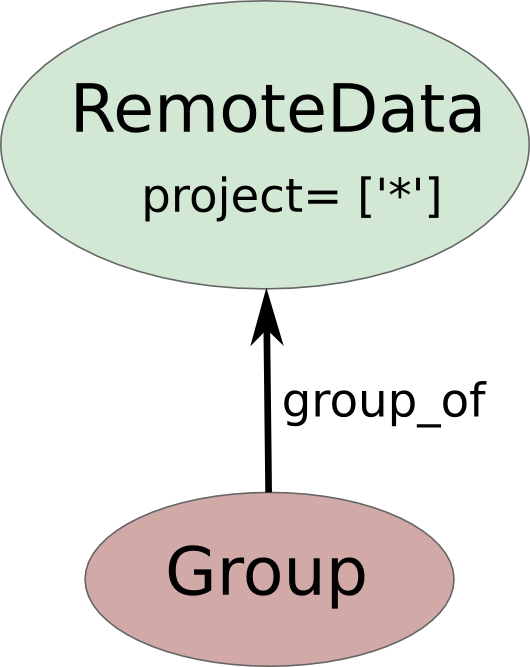
\includegraphics[width=3.5cm]{img/qb_example_1.png}
%~ \end{center}
%~ \caption{Query: Fetch me all the RemoteData that belong to a Group.}
%~ \label{fig:simple_query}
%~ \end{figure}
%
%
There are few details that we should remember from the above query:
\begin{itemize}
\item We \emph{append} to the QueryBuilder instance new entities, and specify how they linked
to previous entities with keywords (``input\_of'', ``output\_of'', ``group\_of'').
The possible relationship keywords can be seen at table~\ref{table:join_rel}.
\item Therefore, we have to \emph{tag} the entities that we want to reference.
We pass these tags along with the keyword, to define a relationship.
\end{itemize}


\begin{table}
	\begin{center}
		\begin{tabular}{l l l l}
		Entity from	& Entity to	& Relationship & Explanation\\ \hline\hline
		Node & Node & input\_of & One node as input of another node\\
		Node & Node & output\_of & One node as output of another node\\
		Node & Node & ancestor\_of & One node as the ancestor of another node\\
		Node & Node & descendant\_of & One node as descendant of another node\\\hline
		Group & Node & group\_of & The group of a node\\
		Node & Group & member\_of & The node is a member of a group\\\hline
		Computer & Node & computer\_of & The computer of a node\\
		Node & Computer & has\_computer & The node of a computer\\\hline
		User & Node & creator\_of & The creator of a node is a user\\
		Node & User & created\_by & The node was created by a user\\
		\end{tabular}
		\caption{Available relationships}
		\label{table:join_rel}
		\end{center}
	\end{table}



\begin{tcolorbox}
\textbf{Exercise:}
\begin{itemize}
	\item Write a query that returns all the StructureData that are an input of a JobCalculation.
\end{itemize}
More (optional) exercises on entity relationships can be found at the appendix.
\end{tcolorbox}


\subsection*{Task 4 - Attributes and extras}
Node and its subclasses have properties stored in key/value format.
These are called \emph{attributes} and \emph{extras} and can be used in filters and projections as the other properties that we have seen previously.

Let's project the value of the property \emph{attributes.energy\_smearing}.
\begin{pythoncommand}
qb = QueryBuilder()
qb.append(
        ParameterData,
        project=["attributes.energy_smearing"]
    )
qb.all()
\end{pythoncommand}
The above query takes the attributes properties of every ParameterData and searches for a
key called energy\_smearing. If that key is found, the value is projected,
otherwise the value is None.  Try it out!
% Of course, searching inside key/values can go as deep as needed.
% E.g. you can project on attributes.a.b.c which will correspond to a property \texttt{\{..., "a": \{... "b": \{... "c": "val" ...\} ...\}, ...\}} % THIS STUFF DOES NOT CORRESPOND TO OUTPUT
~\\~\\
% textcolor{blue}{SZ: What happens with lists?}

\textbf{Hints for the exercises:}
\begin{itemize}
\item If you are unsure about the key of the node that you would like to project, you can print all the attributes of a specific node to get some inspiration. This can be done by calling the \texttt{.get\_attrs()} method of a specific node.
\item The pseudopotentials are stored in AiiDA in with the help of the ORM class UpfData. The element that the pseudopotential correspond to is stored in the \emph{attributes.element} property.
\end{itemize}

\begin{tcolorbox}
\textbf{Exercises:}
\begin{itemize}
	\item Print all the attributes of any ParameterData node stored in your database.
	\item Write a query that checks if you have the pseudopotentials for the element \textit{Si}. Do the same for \textit{C}.
\end{itemize}
More (optional) exercises on attributes and extras can be found at the appendix.
\end{tcolorbox}

%\textcolor{blue}{SZ: Distinct doesn't seem to work on attributes.}

\subsection*{Task 5 - A small ``high-throughput'' analysis}

\begin{figure}[!b]
 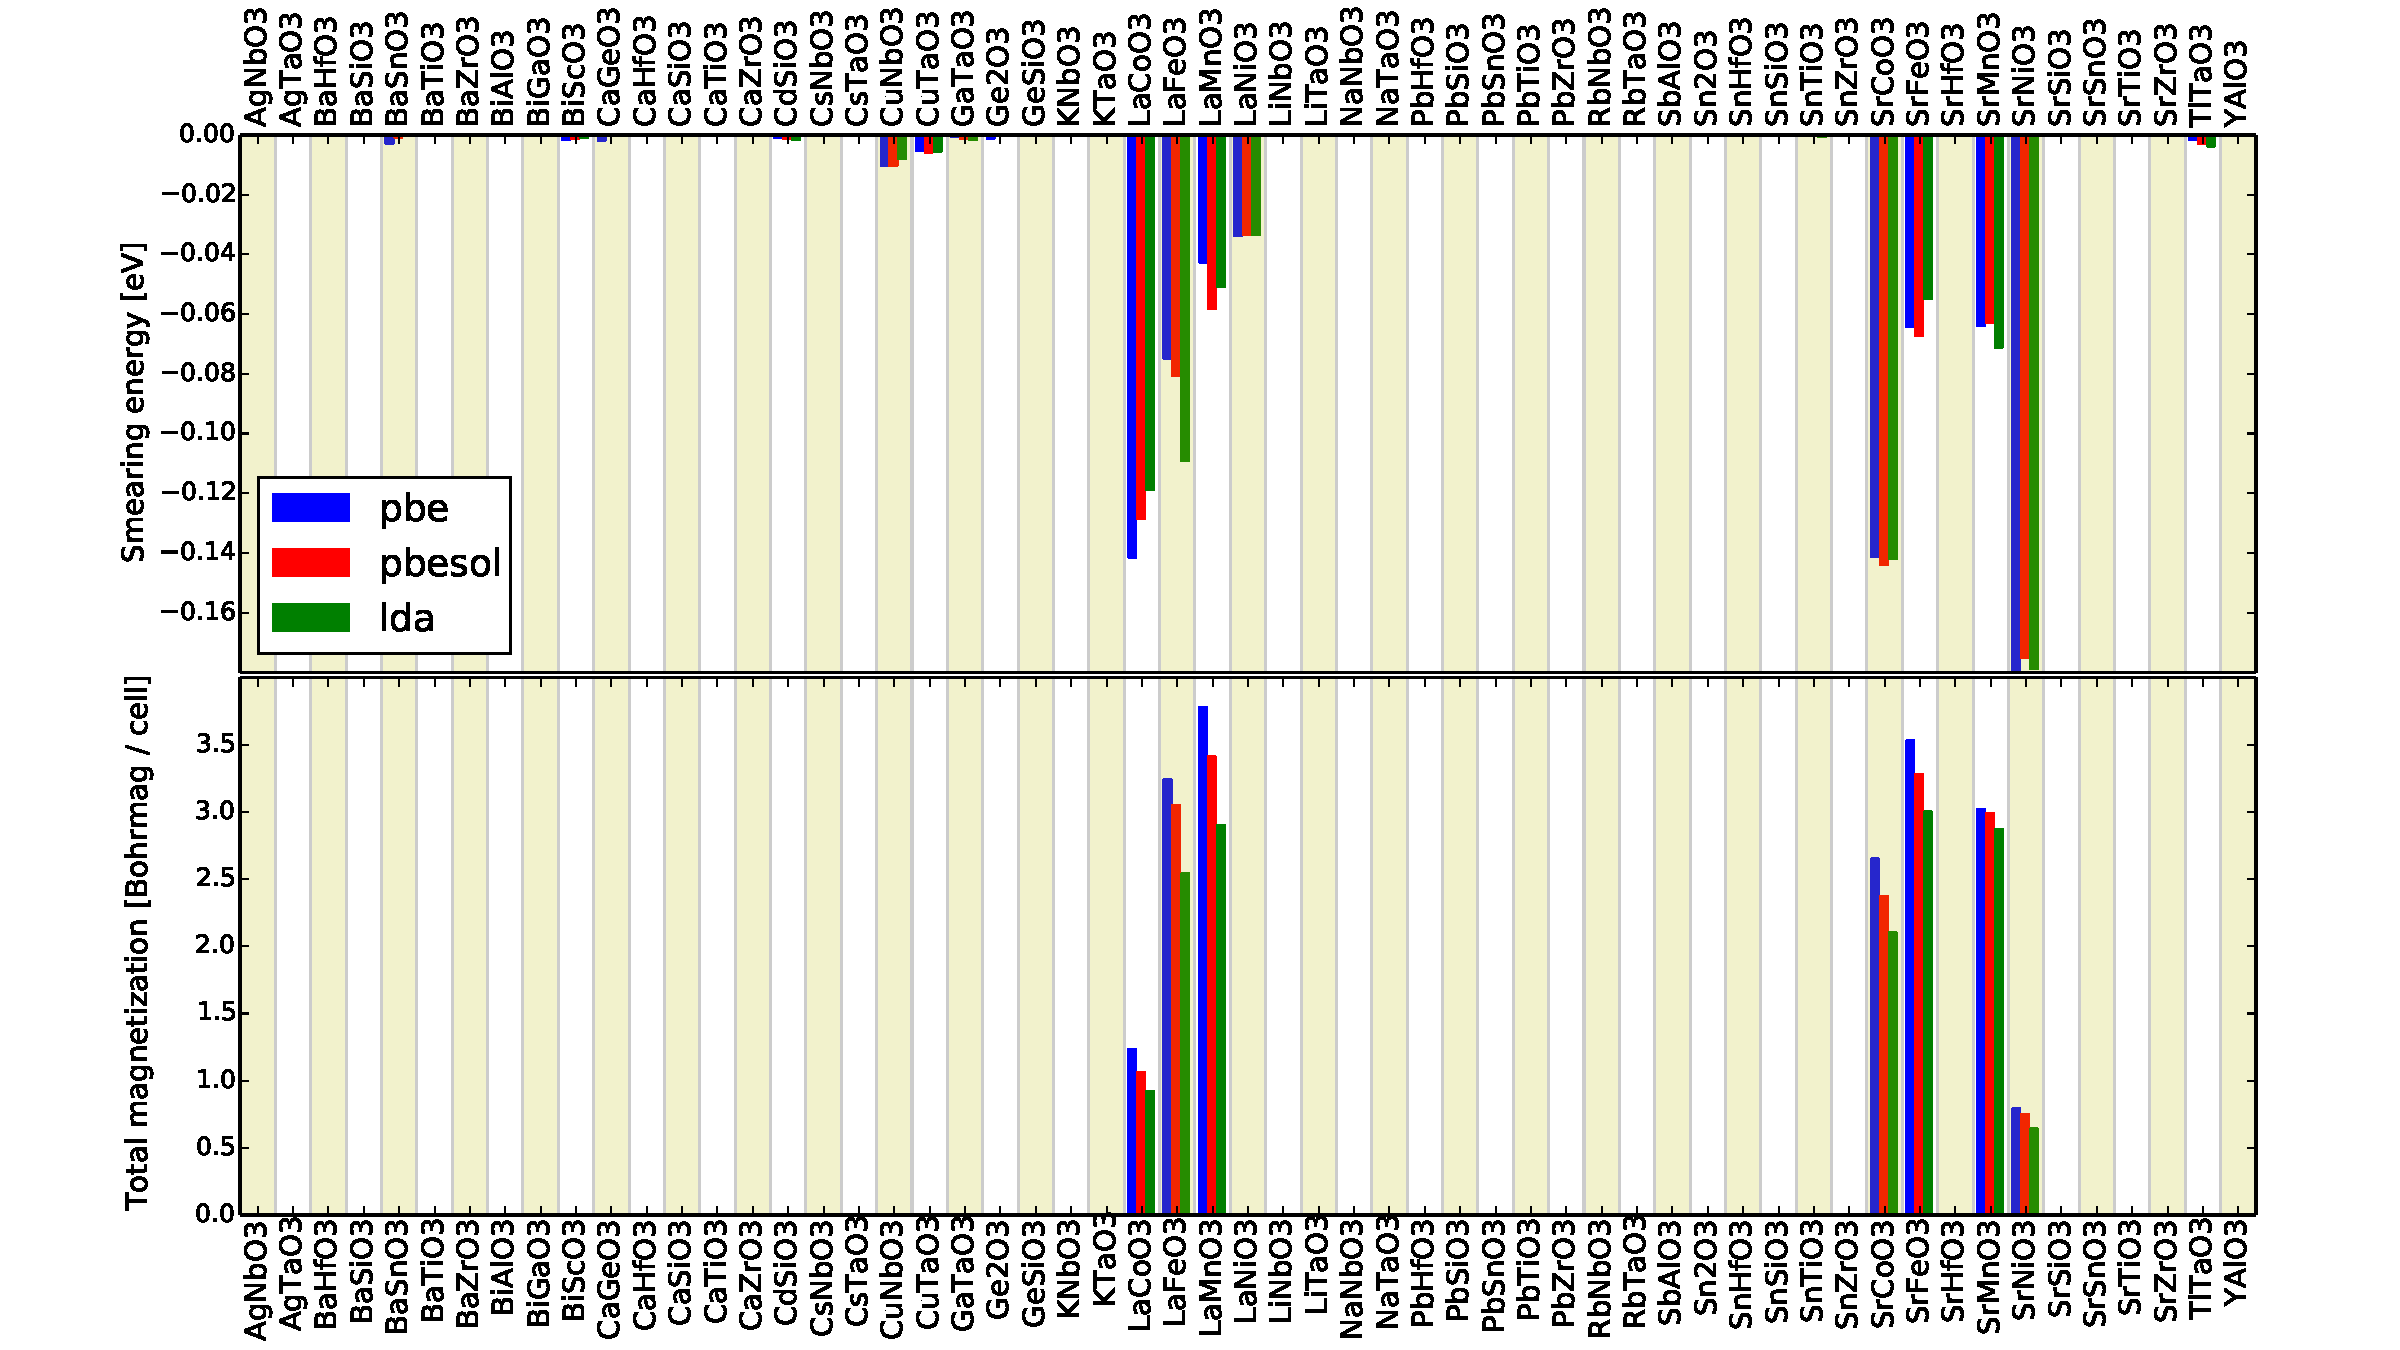
\includegraphics[width=\linewidth]{img/magnetization_smearing_perovskites.pdf}
 \caption{The contribution from the smearing to the total energy (upper) and the magnetization per unit cell (lower)
 in all the perovskites analyzed and for three different pseudopotential families.}
 \label{fig:barplot_perov}
\end{figure}
%
%In the first part of the tutorial, you got an idea of how a single calculation is submitted with AiiDA and how its results can be retrieved, both from the command line and from the \verb|verdi shell|.
In this part of the tutorial, we will focus on how to systematically retrieve, query and analyze the results of multiple calculations using AiiDA.
We know you're able to do this yourself, but to save time, a set of calculations have already been done with AiiDA for you on 57 perovskites,
using three different pseudopotential families (LDA, PBE and PBESOL, all from GBRV 1.2~\cite{ref:GBRV}).
These calculations are spin-polarized (without spin-orbit coupling),
use a Gaussian smearing and perform a variable-cell relaxation of the full unit cell.
The idea of this part of the tutorial is to ``screen'' for magnetic and metallic perovskites in a ``high-throughput'' way.

As you learned in the first part of the tutorial, AiiDA allows to organize calculations in groups.
Once more check the list of groups in your database by typing

\begin{bashcommand}
 verdi group list
\end{bashcommand}

The calculations needed for this task were put in three different groups whose names start with "tutorial\_" (one for each pseudopotential family).
The main task is to make a plot showing, for all perovskites and for each pseudopotential family,
the total magnetization and the $-TS$ contribution from the smearing to the total energy.
An example is shown in \autoref{fig:barplot_perov}.

\subsubsection*{Preparing the analysis}
Let us now guide you through the definition of the query that allows you to retrieve the relevant data.\\~\\
\textbf{Hint for the exercise}:
\begin{itemize}
\item To select multiple names in a filter your filter-dictionary should look like
\begin{pythoncommand}
qb.append(Group, filters={"name": {"in": ["name1","name2","name3"]}})
\end{pythoncommand}
\end{itemize}

\begin{tcolorbox}
\textbf{Exercise:}\\~\\
Please perform the following steps
\begin{enumerate}
\item Write a query to retrieve the three groups and project the respective names.
\item Extend the query to the PwCalculation nodes that are members of the selected groups.
\item Extend the query so that also the chemical formula of the input structure of each calculation is returned.
For simplicity the formulas have been added in the extras of each structure node under the key \textit{"formula"}.
The chemical formula of a StructureData node can also be accessed by the method \cmd{structure.get\_formula()}
\item Every successful PwCalculation has in output a ParameterData instance that stores the results as key-value pairs.
You can find these pairs among the attributes.
To facilitate querying, the parser takes care of storing values always in the same units, and these are documented.
For convenience, the units are also added as key/value pairs (with the same key name, but with \cmd{\_units}  appended).
% Load a ParameterData node (ex. pk=3516) and find the keys that you are interested in by typing:
% \begin{pythoncommand}
% node.get_attrs()
% \end{pythoncommand}
Extend the query so that also the output ParameterData of each calculation is returned.
Project only the attributes relevant to your analysis (like smearing energy, ...).
\end{enumerate}
\end{tcolorbox}

\subsubsection*{Running the query and plotting the results}

% We will now get into a small high-throughput analysis of a larger number of PwCalculations.
% The goal is to extend the above query so that you project also on the resulting magnetization, smearing, and group name of the group they belong to.
Now that your query is ready just run it:
\begin{pythoncommand}
 res = qb.dict()
\end{pythoncommand}
The above results returns a list of dictionaries.
In order to be able to plot the data that you have retrieved a script called \texttt{plot\_calculation\_results.py}
was provided to you. This script reads an input text file containing the data and produces a plot similar to \autoref{fig:barplot_perov}.

You should prepare this input text file in the following format,
formatting the data present in \texttt{res}.
Each row in the input file represents one calculation and contains the following informations separated by a comma:

\begin{enumerate}
\item The structure formula.
\item The name of the pseudo family. Remove the tutorial\_ substring from the name if it bothers you.
\item The smearing energy
\item The unit used for the smearing energy.
\item The magnetization.
\item The unit of the magnetization.
\end{enumerate}

As an example, the first three lines can look like:
\begin{bashcommand}
Sn2O3,  pbesol, -1.95921960844e-05,  eV,  0.0,  Bohrmag / cell
CaSiO3,    pbe,                0.0,  eV,  0.0,  Bohrmag / cell
CuNbO3,    pbe,    -0.010202636111,  eV,  0.0,  Bohrmag / cell
\end{bashcommand}

%Once this is done, you can read the this file with the provided script.


\iffalse
You should be able to print the data in the desired format with about ten lines of python code. In case you are not very familiar with python, you may take inspiration from the following snippet:

\begin{pythoncommand}
with open("res.txt","w") as fout:
  for row in res:
    formula = row["structure"]["extras.formula"]
    magnetization = row["results"]["attributes.total_magnetization"]
    magnetization_units = row["results"]["attributes.total_magnetization_units"]
    smearing = row["results"]["attributes.energy_smearing"]
    smearing_units = row["results"]["attributes.energy_smearing_units"]
    pseudo_family = row["group"]["name"].replace("tutorial_", "")
    str_row = ", ".join(
            map(str, (formula, pseudo_family,
            smearing, smearing_units, magnetization, magnetization_units
        ))
    	)
    fout.write("{}\n".format(str_row))

\end{pythoncommand}
\fi


If you are producing the desired output, write that output to a file (here we will call it \texttt{res.txt}).
If you are using \emph{jupyter}, you can plot the files and see the results directly in the browser. First, in a cell, do
\begin{pythoncommand}
cd ~/tutorial_scripts/
\end{pythoncommand}
to go to the right folder, and then in the following cell type:
\begin{pythoncommand}
%pylab inline
import plot_calculation_results
plot_calculation_results.plot_results('../res.txt')
\end{pythoncommand}
(possibly replacing \texttt{../res.txt} with the correct location of the file).

Otherwise, if you are not using \emph{jupyter}, to plot your data just go in the shell and change directory to the subfolder \texttt{tutorial\_scripts}. Then type in the shell
\begin{bashcommand}
python plot_calculation_results.py ../res.txt
\end{bashcommand}
(or replace \texttt{../res.txt} with the correct location of the \texttt{res.txt} file). The \texttt{plot\_calculation\_results.py} file is already provided to you among the scripts given to you for the tutorial, in the \texttt{tutorial\_scripts} folder. If everything is right, you should get a plot similar to \autoref{fig:barplot_perov}.
You can also pass an option to store the output as a plot on a file:
\begin{bashcommand}
python plot_calculation_results.py res.txt -o myresult.pdf
\end{bashcommand}


\begin{tcolorbox}
\textbf{Exercise:}
\begin{itemize}
\item Look at the plot that you produced. Which of the perovskites are metals?
\end{itemize}
\end{tcolorbox}


%~ \begin{pythoncommand}
%~ qb = QueryBuilder()
%~ qb.append(StructureData, project="*")
%~ qb.append(Calculation, tag="calc")
%~ qb.append(
		%~ ParameterData,
		%~ project="attributes.energy",
		%~ filters={"attributes.energy":{"<=":0}}
	%~ )
%~ qb.append(Group, group_of="calc")
%~
%~ for structure, energy in qb.iterall():
    %~ print structure.get_formula(), energy
%~ \end{pythoncommand}


%~ Figures~\ref{fig:barplot_mag} and~\ref{fig:barplot_smearing} show the plots you should obtain (note that in Fig.~\ref{fig:barplot_smearing} we actually plotted $|-TS|=TS$ since $-TS$ is negative for all the species studied).

%

%\begin{figure}[tb]
% 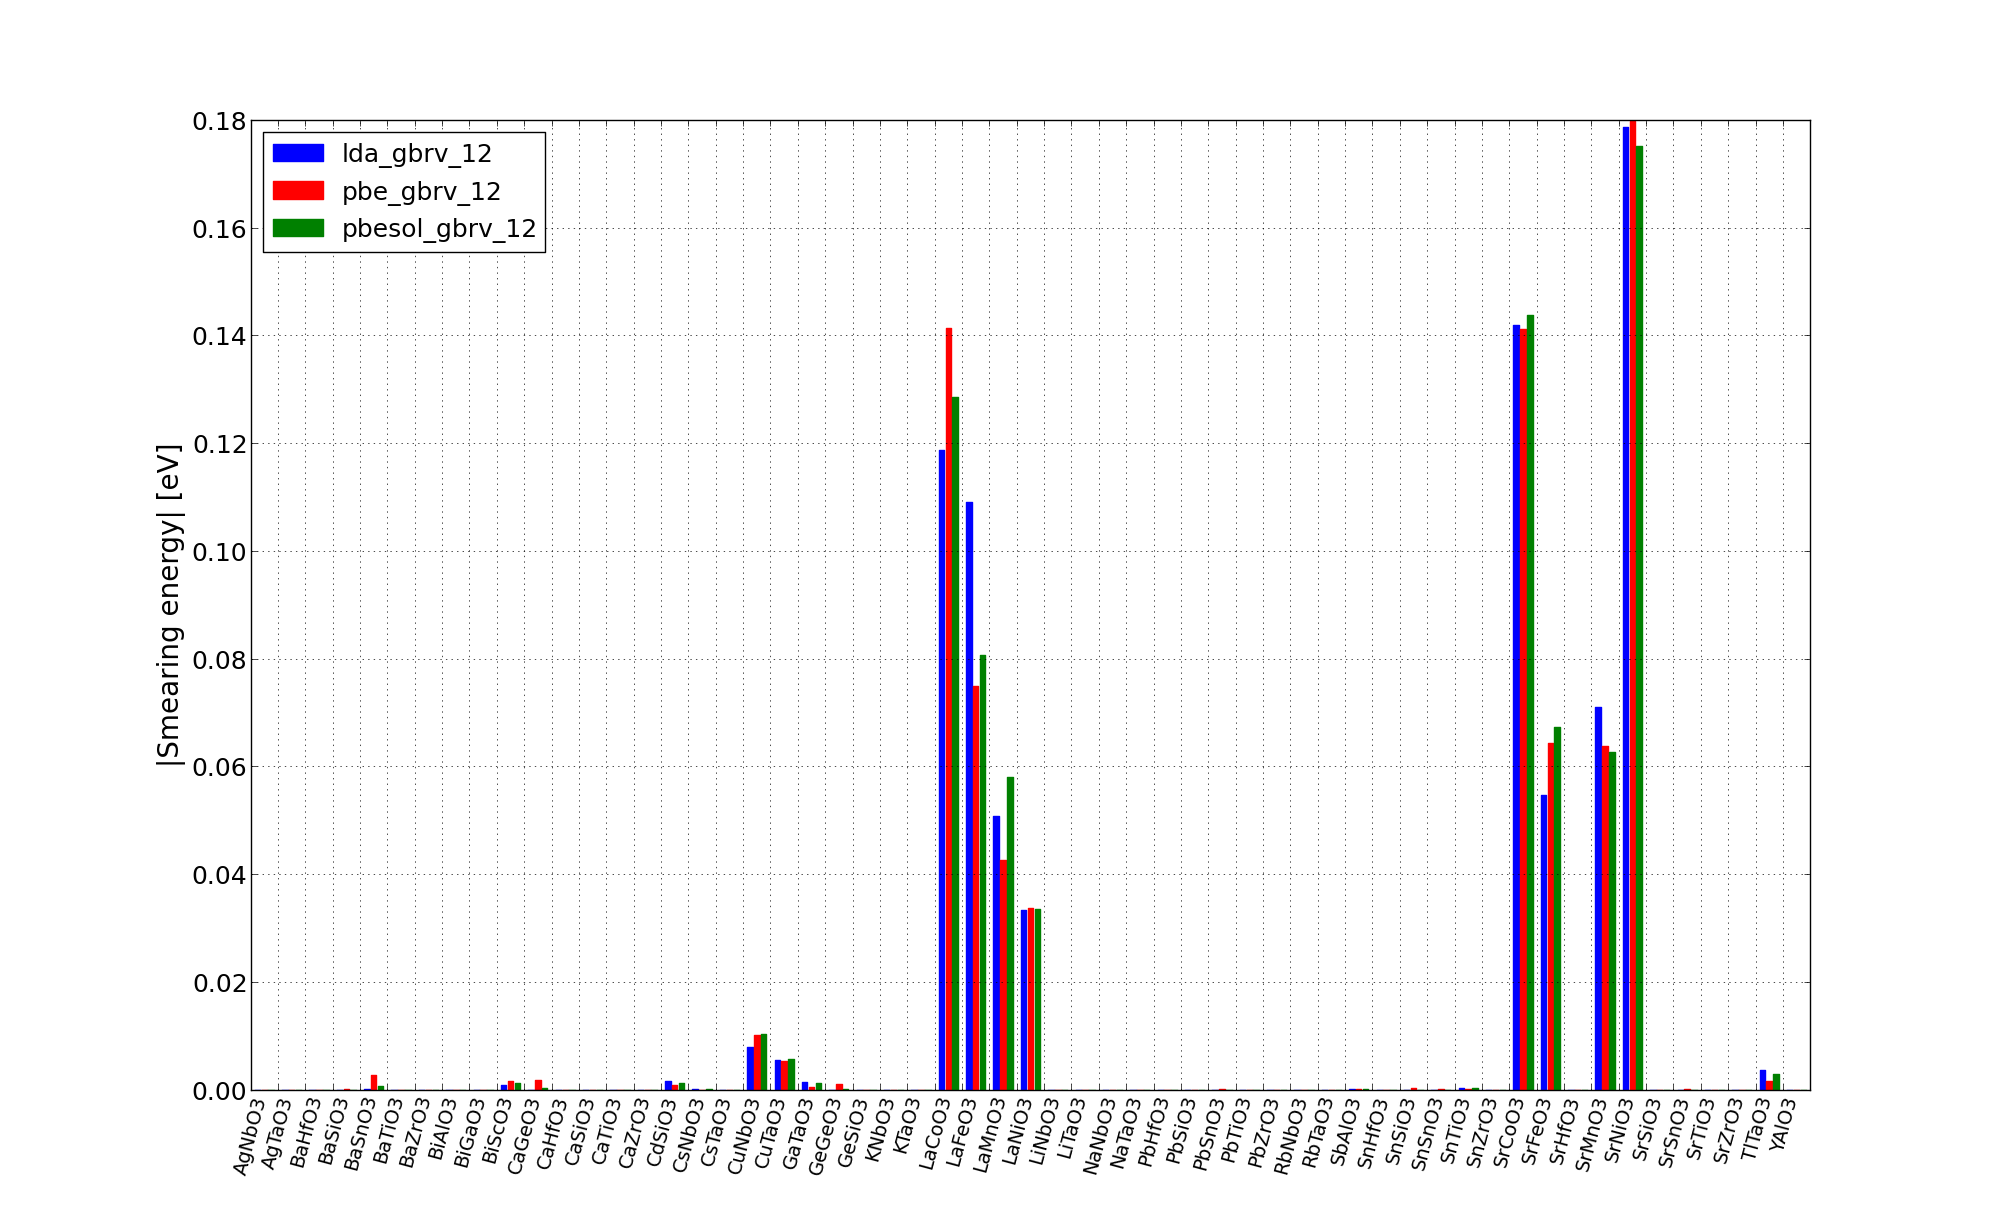
\includegraphics[width=\linewidth]{img/smearing_energy_vs_perovskites_allpseudo_Gaussian_0p02.png}
% \caption{$-TS$ contribution to the total energy (in absolute value, since it is actually negative for all species) from the smearing, for all the perovskites analyzed and for three different pseudopotential families\label{fig:barplot_smearing}.}
%\end{figure}
%
%Two python scripts can help you doing this (you can find them in the subfolder \texttt{$\sim$/tutorial\_scripts}):
%\begin{itemize}
%\item \texttt{get\_pks.py}: gives a list of pk numbers for a given group, possibly filtering also for those perovskites with given ``A"" and/or ``B"" species.
%
%Use it from the command line in the following way:
%\begin{bashcommand}
% ./get_pks.py <group_name> -A <A_element> -B <B_element>
%\end{bashcommand}
%This script prints on output the list of pks (first column) and chemical formulas (second column) of the perovskite(s). The \cmd{-A} and \cmd{-B} options are optional.
% \item \texttt{get\_info.py}: prints several information about a given calculation.
%
%You can use it (from a terminal) with the command
%\begin{bashcommand}
% ./get_info.py <pk_number>
%\end{bashcommand}
%\end{itemize}
%%
%We suggest that you give a look to the content of the scripts we provide, to understand what they do. To prepare the plots, you can either create your own python script taking inspiration from the two scripts that we provide, or (if you do not want to write a Python script, but rather use bash commands) you can simply use the provided scripts as they are.
%Note also that if the graphical plotting software is too slow to load over SSH, you can create a text data file on the remote machine, then copy the data on your computer, and prepare the plot there (you can use any software you like: gnuplot, xmgrace, or even simply Excel).


%~ \subsection*{Task 5.2}
%~ We chose five calculations (using the PBEsol pseudopotential family) of five different representative perovskites, for which we plotted the $-TS$ contribution as a function of the Kohn-Sham band-gap. The resulting plot is shown in \cref{fig:smearing_vs_bandgaps}. \begin{tcolorbox}
%~ Use this plot and the plots you obtained for the smearing energy of all perovskites, to define a criterion to distinguish which compounds are metals and which ones are insulators.
%~ \end{tcolorbox}

%
%\begin{figure}[tb]
% \centering
% 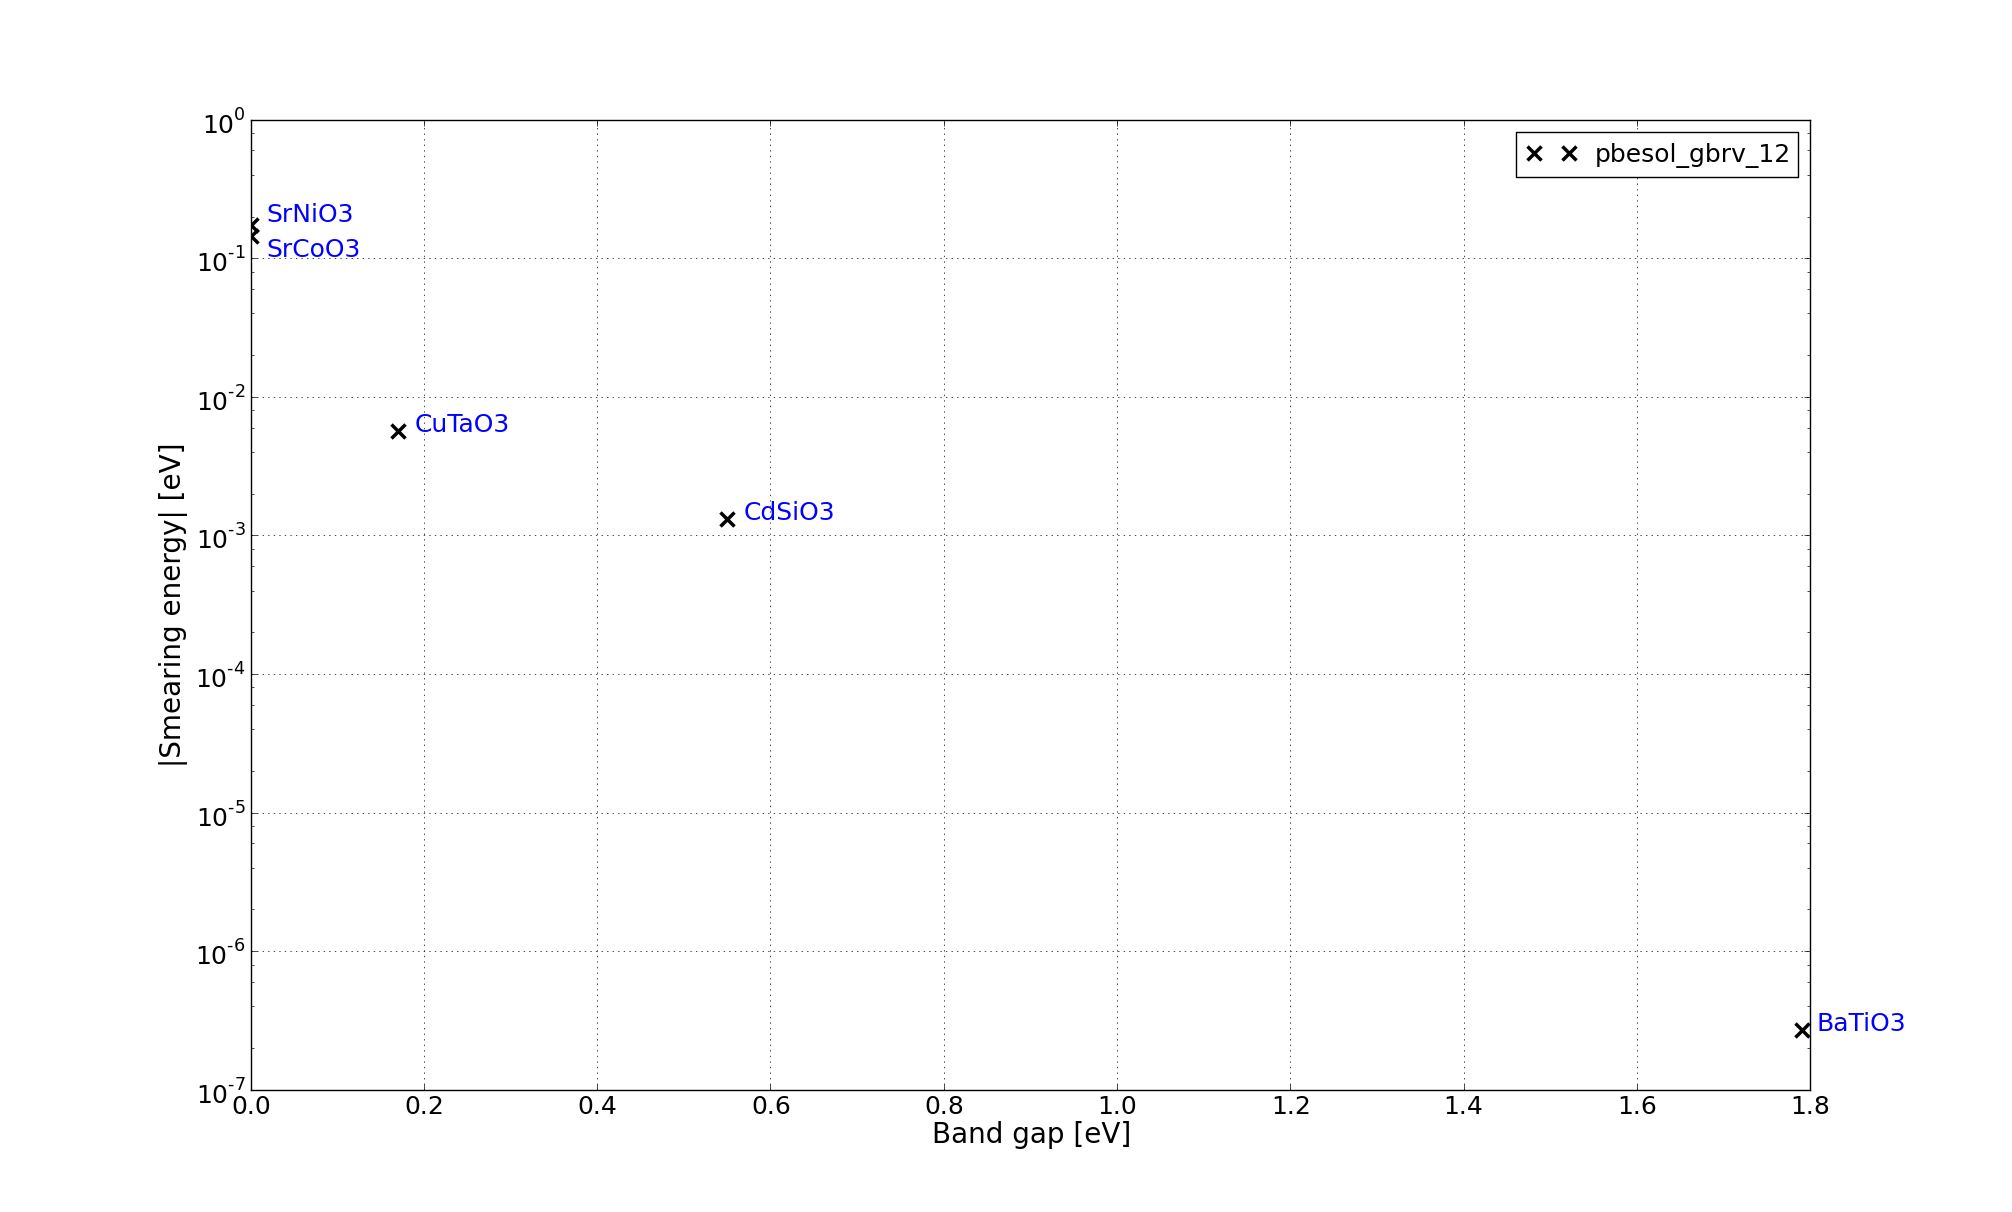
\includegraphics[width=0.7\linewidth]{img/smearing_energy_vs_bandgap_Gaussian_0p02.png}
% \caption{$-TS$ contribution (in absolute value) vs. Kohn-Sham band-gap for five selected perovskites, using the pseudopotentials with PBEsol functional\label{fig:smearing_vs_bandgaps}.}
%\end{figure}
%

%~ \subsection*{Task 5.3}
%~ Finally, we want to print the list of perovskites which are metals according to the criterion we defined, and those that are magnetic. To this aim, we can use the \emph{QueryBuilder} that helps you making easy queries to the database, without the need of knowing the SQL language.



%~ \begin{tcolorbox}
%~ Do another query to find out metallic perovskites according to the criterion on the smearing energy you found above. Check that your query results are consistent with the plots you did at the beginning of the exercise.
%~ \end{tcolorbox}

%}{
% Version using the Jupyter Notebook

\section{Queries in AiiDA: The QueryBuilder}
\label{sec:querybuilder}

\begin{tcolorbox}
This part of the tutorial is provided only in interactive mode through a Jupyter notebook, which you will be able to run in your browser.
To accomplish this we first need to start the Jupyter server, if you didn't do it already at the very beginning of the tutorial.
First make sure you are connected to the virtual machine with local forwarding enabled, as described in section \ref{sec:sshintro}.
Then, on the virtual machine, first make sure your are in the \texttt{aiida} virtual environment:

\begin{bashcommand}
workon aiida
\end{bashcommand}

If the virtual environment is successfully loaded, your prompt should be prefixed with \texttt{(aiida)}.
To finally launch the Jupyter server, execute the following commands:

\begin{bashcommand}
cd ~/examples/aiida-demos/tutorial/
jupyter notebook --no-browser
\end{bashcommand}

If all went well, you should now be able to open up a browser on your local machine and point it to the following address \texttt{http://localhost:8888/?token=2a3ba3...} (replace the token with the one printed on output by the previous command).
This should now show you a directory navigator.
To open the notebook, click on \texttt{querybuilder} and then select the file \texttt{tutorial.ipynb}.
Note that there is also a \texttt{solution.ipynb}, which is a copy of the same notebook, but which contains the solutions to all the exercises.
You can use this version at your own discretion if you get stuck at some point (but we suggest that you try not to look at it at first).
\end{tcolorbox}

%}
% !TEX root = ../AiiDA_tutorial.tex
%%%%%%%%%%%%%%%%This slot is devoted to workflows, although the material inherited from the old tutorial does not use them.
% Nevertheless, it has been suggested to use workflows for calculating equation of state, so all this stuff can be inspirational 
%%%%%%%%%%%%%%%%%%%%%%

\section{AiiDA Workflows: workfunctions, workchains}

The aim of the last part of this tutorial is to introduce the concept of workflows in AiiDA. 

In this section, we will ask you to:
\begin{enumerate}
\item Understand how to keep the provenance when running small python scripts to convert one data object into another (postprocessing, preparation of inputs, \ldots)
\item Understand how to represent simple python functions in the AiiDA database
\item Learn how to write a simple workflow in AiiDA (without and with remote calculation submission)
\item Learn how to write a workflow with checkpoints: this means that, even if your
workflows requires external calculations to start, them and their dependences are managed through the daemon. While you are waiting for the calculations to complete, you can stop and even shutdown the computer in which AiiDA is running. When you restart, the workflow will
continue from where it was.
\item (optional) Go a bit deeper in the syntax of workflows with checkpoints (WorkChain), e.g. implementing a convergence workflow using \texttt{while} loops.
\end{enumerate}

A note: this is probably the most ``complex'' part of the tutorial.
We suggest that you try to understand the underlying logic behind the scripts,
without focusing too much on the details of the workflows implementation or the syntax.
If you want, you can then focus more on the technicalities in a second reading.

\subsection[Workfunctions]{Introduction}
The ultimate aim of this section is to create a workflow to calculate the equation of state of silicon. This is a very common task for an \textit{ab initio} researcher. An equation of state consists in calculating the total energy $E$ as a function of the unit cell volume $V$. The minimal energy is reached at the equilibrium volume $V^{\star}$. Equivalently, the equilibrium is defined by a vanishing pressure $p=-dE/dV$. In the vicinity of the minimum, the functional form of the equation of state can be approximated by a parabola. Such an approximation greatly simplifies the calculation of the bulk modulus, that is proportional to the second derivative of the energy $d^2E/dV^2$ (a more advanced treatment requires fitting the curve with, e.g., the Birch--Murnaghan expression).

The process of calculating an equation of state puts together several operations. 
First, we need to define and store in the AiiDA database the basic structure of, e.g., bulk Si.
Next, one has to define several structures with different lattice parameters. Those structures must be connected between them in the database, in order to ensure that their provenance is recorded. In other words, we want to be sure that in the future we will know that if we find a bunch of rescaled structures in the database, they all descend from the same one. How to link two nodes in the database in a easy way is the subject of Sec.~\ref{sec:provenancewf}.

In the following sections, the newly created structures will then serve as an input for total energy calculations performed, in this tutorial, with Quantum ESPRESSO. This task is very similar to what you have done in the previous part of the tutorial. Finally, you will fit the resulting energies as a function of volume to get the bulk modulus.
As the EOS task is very common, we will show how to automate its computation with workflows, and how to deal with both serial and parallel (i.e., independent) execution of multiple tasks. Finally, we will show how to introduce more complex logic in your workflows such as loops and conditional statements (Sec.~\ref{sec:convpressure}), with an example on a convergence loop to find iteratively the minimum of an EOS.


\subsection[Workfunctions]{\label{sec:provenancewf}Workfunctions: a way to generalize provenance in AiiDA}


%Figure with workfunction graph
\begin{figure}[!th]
\centering
 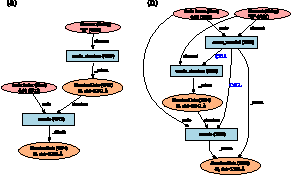
\includegraphics[width=\linewidth]{img/workfunctions}
 \caption{ \label{Fig:workfunctions}Typical graphs created by using a workfunction. (a) The workfunction ``create\_structure'' takes a \texttt{Str} object as input and returns a single \texttt{StructureData} object which is used as input for the workfunction ``rescale'' together with a \texttt{Float} object. This latter workfunction returns another \texttt{StructureData} object, defining a crystal having the rescaled lattice constant. (b) Graph generated by nesting workfunctions. A wrapper workfunction ``create\_rescaled" calls serially ``create\_structure'' and ``rescale". This relationship is stored via ``CALL'' links.}
\end{figure}


Imagine to have a function that takes as input a string of the name of a chemical element and generates the corresponding bulk structure as a \texttt{StructureData} object. The function might look like this (you will find this function in the folder \texttt{/home/aiida/tutorial\_scripts/create\_rescale.py} on your virtual machine):

\begin{pythoncommand}
def create_diamond_fcc(element):
    """
    Workfunction to create the crystal structure of a given element.
    For simplicity, only Si and Ge are valid elements.
    :param element: The element to create the structure with.
    :return: The structure.
    """
    import numpy as np
    elem_alat= {
                "Si": 5.431, # Angstrom
                "Ge": 5.658,
               }

    # Validate input element
    symbol = str(element)
    if symbol not in elem_alat.keys():
       raise ValueError("Valid elements are only Si and Ge")

    # Create cel starting having lattice parameter alat corresponding to the element
    alat = elem_alat[symbol]
    the_cell = np.array([[0., 0.5, 0.5],
                         [0.5, 0., 0.5],
                         [0.5, 0.5, 0.]]) * alat

    # Create a structure data object
    StructureData = DataFactory("structure")
    structure = StructureData(cell=the_cell)
    structure.append_atom(position=(0., 0., 0.), symbols=str(element))
    structure.append_atom(position=(0.25*alat, 0.25*alat, 0.25*alat),
                          symbols=str(element))
    return structure
\end{pythoncommand}

For the equation of state you need another function that takes as input a \texttt{StructureData} object and a rescaling factor, and returns a \texttt{StructureData} object with the rescaled lattice parameter (you will find this function in the same file \texttt{create\_rescale.py} on your virtual machine):

\begin{pythoncommand}
def rescale(structure, scale):
    """
    Workfunction to rescale a structure

    :param structure: An AiiDA structure to rescale
    :param scale: The scale factor (for the lattice constant)
    :return: The rescaled structure
    """
    the_ase = structure.get_ase()
    new_ase = the_ase.copy()
    new_ase.set_cell(the_ase.get_cell() * float(scale), scale_atoms=True)
    new_structure = DataFactory('structure')(ase=new_ase)
    return new_structure
\end{pythoncommand}

In order to generate the rescaled starting structures, say for five different lattice parameters you would combine the two functions. Enter the following commands in the \texttt{verdi shell} from the \texttt{tutorial\_scripts} folder.  

\begin{pythoncommand}
from create_rescale import create_diamond_fcc, rescale

s0 = create_diamond_fcc("Si")
rescaled_structures = [rescale(s0, factor) for factor 
                      in (0.98, 0.99, 1.0, 1.1, 1.2)]
\end{pythoncommand}

and store them in the database:

\begin{pythoncommand}
s0.store()
for struct in rescaled_structures:
   struct.store()
\end{pythoncommand}

\begin{tcolorbox}
Run the commands above to store all the structures.
\end{tcolorbox}

As expected, all the structures that you have created are not linked in any manner as you can verify via the \cmd{get\_inputs()/get\_outputs()} methods of the StuctureData class.
Instead, you would like these objects to be connected as sketched in Fig.~\ref{Fig:workfunctions}a. Now that you are familiar with AiiDA, you know that the way to connect two data nodes is through a calculation.
%However, you do not want to run such simple python functions on a cluster! Rather, you would like to simply run  them as simple python functions, but keep at the same time the provenance.
In order to ``wrap'' python functions and automate the generation of the
needed links, in AiiDA we provide you with what we call ``workfunctions''. A normal function can be converted to a workfunction by using the \texttt{@workfunction} decorator\footnote{In simple (or even simplified) words, a decorator is a function that modifies the behavior of another function. In python, a function can be decorated by adding a line of the form \texttt{@decorating\_function\_name} on the line just before the \texttt{def} line of the decorated function. If you want to know more, there are many online resources explaining python decorators.} that takes care of storing the execution as a calculation and adding the links between the input and output data nodes.

\begin{tcolorbox}
In our case, what you need to do is to modify the two functions as follows (note that we import \texttt{workfunction} as \texttt{wf} to be shorter, but this is not required). You can do it in the file \texttt{create\_rescale.py}:
\end{tcolorbox}

\begin{pythoncommand}
# Add this import
from aiida.work import workfunction as wf
 
# Add decorators
@wf
def create_diamond_fcc(element):
    ...
    ...
 
@wf
def rescale(structure, scale):
    ...
    ...
\end{pythoncommand}

\emph{Important}: when you use workfunctions, you have to make sure that their input and output are actually Data nodes, so that they can be stored in the database. AiiDA objects such as \texttt{StructureData}, ParameterData, etc.\@ carry around information about their provenance as stored in the database. This is why we must use the special database-storable types Float, Str, etc.\@ as shown in the snippet below.

\begin{tcolorbox}
Try now to run the following script:
\end{tcolorbox}
\begin{pythoncommand}
from aiida.orm.data.base import Float, Str
from create_rescale import create_diamond_fcc, rescale

s0 = create_diamond_fcc(Str("Si"))
rescaled_structures = [rescale(s0,Float(factor)) for factor in (0.98, 0.99, 1.0, 1.1, 1.2)]
\end{pythoncommand}
and check now that the output of \texttt{s0} as well as the input of the rescaled structures point to an intermediate ProcessCalculation node, representing the execution of the
workfunction, see Fig.~\ref{Fig:workfunctions}. 
\begin{tcolorbox}
For instance, you can check that the output links of \texttt{s0} are the five \texttt{rescale} calculations:
\end{tcolorbox}
\begin{pythoncommand}
s0.get_outputs()
\end{pythoncommand}
which outputs
\begin{pythoncommand}
[<FunctionCalculation: uuid: 01b0b137-974c-4d80-974f-ea4978b12019 (pk: 4970)>,
 <FunctionCalculation: uuid: 1af5ead6-0ae0-42a7-969c-1f0e88300f4a (pk: 4973)>,
 <FunctionCalculation: uuid: 22dee9d5-0382-48a3-9319-e800506946f1 (pk: 4976)>,
 <FunctionCalculation: uuid: dc4c93b7-3e7a-4f51-8d44-cf15c5707ddb (pk: 4979)>,
 <FunctionCalculation: uuid: f5b4e9f2-0d50-4b3d-a76b-7a12d232ea54 (pk: 4982)>]
\end{pythoncommand}
\begin{tcolorbox}
and the inputs of each ProcessCalculation (``rescale'') are obtained with:
\end{tcolorbox}
\begin{pythoncommand}
for s in s0.get_outputs():
     print s.get_inputs()
\end{pythoncommand}
that will return
\begin{pythoncommand}    
[0.98, <StructureData: uuid: 9b76b5fa-2908-4f88-a4fb-7a9aa343a1f3 (pk: 4968)>]
[0.99, <StructureData: uuid: 9b76b5fa-2908-4f88-a4fb-7a9aa343a1f3 (pk: 4968)>]
[1.0, <StructureData: uuid: 9b76b5fa-2908-4f88-a4fb-7a9aa343a1f3 (pk: 4968)>]
[1.1, <StructureData: uuid: 9b76b5fa-2908-4f88-a4fb-7a9aa343a1f3 (pk: 4968)>]
[1.2, <StructureData: uuid: 9b76b5fa-2908-4f88-a4fb-7a9aa343a1f3 (pk: 4968)>]
\end{pythoncommand}

\subsubsection{Workfunction nesting}
One key advantage of workfunctions is that they can be nested, namely, a workfunction can invoke workfunctions inside its definition, and this ``call'' relationship will also be automatically recorded in the database. 
As an example, let us combine the two previously defined workfunctions by means of a wrapper workfunction called ``create\_rescaled'' that takes as input the element and the rescale factor.
\begin{tcolorbox}
Type in your shell (or modify the functions defined in \texttt{create\_rescale.py} and then run):
\end{tcolorbox}
%%%%%%%%%%Call link
\begin{pythoncommand}
@wf
def create_rescaled(element, scale):
    """
    Workfunction to create and immediately rescale
    a crystal structure of a given element.
    """
    s0 = create_diamond_fcc(element)
    return rescale(s0,scale)
\end{pythoncommand}
and create an already rescaled structure by typing 
\begin{pythoncommand}
s1 = create_rescaled(element=Str("Si"), scale=Float(0.98))
\end{pythoncommand}
\begin{tcolorbox}
Now inspect the input links of \texttt{s1}:
\end{tcolorbox}
\begin{pythoncommand}
In [6]: s1.get_inputs()
Out[6]: 
[<FunctionCalculation: uuid: a672317b-3091-4135-9d84-12c2fff34bfe (pk: 5005)>,
 <FunctionCalculation: uuid: a672317b-3091-4135-9d84-12c2fff34bfe (pk: 5005)>,
 <FunctionCalculation: uuid: f64f4a70-70ff-4551-ba4d-c186328d8bd6 (pk: 5002)>]
\end{pythoncommand}

The object \texttt{s1} has three incoming links, corresponding to \emph{two} different calculations as input (in this case, pks 5002 and 5005). These correspond to the calculations ``create\_rescaled'' and ``rescale'' as shown in Fig.~\ref{Fig:workfunctions}b.
It is normal that calculation 5005 has two links, don't worry about that\footnote{If you are curious: the two links have the same label, but are of different \emph{link\_type}: one is a \textbf{create} link, that keeps track of the calculation that actually generated the node. Instead the other one is of type \textbf{return}, stating that the workfunction, beside creating that node, also returned it as an output. Calculation 5002 instead only returned the node but it did not generate it, therefore there is only one link between it and the final \texttt{StructureData}.}.
To see the ``call'' link, inspect now the outputs of the calculation appearing only once in the list. Write down its \texttt{<pk>} (in general, it will be different from 5002), then in the shell load the corresponding node and inspect the outputs:
\begin{pythoncommand}
In [12]: p1 = load_node(<pk>)
In [13]: p1.get_outputs_dict()
\end{pythoncommand}
\begin{tcolorbox}
You should be able to identify the two ``children" calculations as well as the final structure (you will see the calculations linked via CALL links: these are calculation-to-calculation links representing the fact that \texttt{create\_rescaled} called two sub-workfunctions). The graphical representation of what you have in the database should match Fig.~\ref{Fig:workfunctions}b.  
\end{tcolorbox}

\subsection{\label{sec:sync} Run a simple workflow}

Let us now use the workfunctions that we have just created to build a simple workflow to calculate the equation of state of silicon. We will consider five different values of the lattice parameter obtained rescaling the experimental minimum, $a=5.431~\text{\AA}$, by a factor in $[0.96, 0.98, 1.0, 1.02, 1.04]$. We will write a simple script that runs a series of five calculations and at the end returns the volume and the total energy corresponding to each value of the lattice parameter. For your convenience, besides the functions that you have written so far in the file \texttt{create\_rescale.py}, we provide you with some other utilities to get the correct pseudopotential and to generate a pw input file, in the module \texttt{common\_wf.py} which has been put in the \texttt{tutorial\_scripts} folder.

\begin{tcolorbox}
We have already created the following script named \texttt{simple\_sync\_workflow.py}, which you are free to look at but please go through the lines carefully and make sure you understand them.
If you decide to create your own new script, make sure to also place it in the folder \texttt{tutorial\_scripts}, otherwise the imports won't work.
\end{tcolorbox}
Besides the functions in the local folder
\begin{pythoncommand}
from create_rescale import create_diamond_fcc, rescale
from common_wf import generate_scf_input_params
\end{pythoncommand}
you need to import few further AiiDA classes and functions:
\begin{pythoncommand}
from aiida.work import run, Process
from aiida.work import workfunction as wf
from aiida.orm.data.base import Str, Float
from aiida.orm import CalculationFactory, DataFactory
\end{pythoncommand}

The only imported function that deserves an explanation is \texttt{run}.
For the time being, you just need to know that it is a function that needs to be used to execute a new workflow.
The actual body of the script is the following.
We suggest that you first have a careful look at it before running it.

\begin{pythoncommand}
# Load the calculation class 'PwCalculation' using its entry point 'quantumespresso.pw'
PwCalculation = CalculationFactory('quantumespresso.pw')

scale_facs = (0.96, 0.98, 1.0, 1.02, 1.04)
labels = ["c1", "c2", "c3", "c4", "c5"]

@wf
def run_eos_wf(codename, pseudo_family, element):
    print "Workfunction node identifiers: {}".format(Process.current().calc)
    s0 = create_diamond_fcc(Str(element))

    calcs = {}
    for label, factor in zip(labels, scale_facs):
        s = rescale(s0, Float(factor))
        inputs = generate_scf_input_params(s, str(codename), Str(pseudo_family))
        print "Running a scf for {} with scale factor {}".format(element, factor)
        result = run(PwCalculation, **inputs)
        print "RESULT: {}".format(result)
        calcs[label] = get_info(result)

    eos = []
    for label in labels:
        eos.append(calcs[label])

    # Return information to plot the EOS
    ParameterData = DataFactory("parameter")
    retdict = {
            'initial_structure': s0,
            'result': ParameterData(dict={'eos_data': eos})
        }

    return retdict
\end{pythoncommand}

If you look into the previous snippets of code, you will notice that the way we submit a QE calculation is slightly different from what you have seen in the first part of the tutorial.  The following:
\begin{pythoncommand}
result = run(PwCalculation, **inputs)
\end{pythoncommand}
runs in the current python session (without the daemon), waits for its completion and returns the output in the user-defined variable \texttt{result}.
The latter is a dictionary whose values are the output nodes generated by the calculation, with the link labels as keys.
For example, once the calculation is finished, in order to access the total energy, we need to access the ParameterData node which is linked via the ``output\_parameters'' link (see again Fig.~1 of Day 1 Tutorial, to see inputs and outputs of a Quantum ESPRESSO calculation).
Once the right node is retrieved as \cmd{result[`output\_parameters']}, we need to get the \texttt{energy} attribute. The global operation is achieved by the command
\begin{pythoncommand}
result['output_parameters'].dict.energy
\end{pythoncommand}
As you see, the function \texttt{run\_eos\_wf} has been decorated as a workfunction to keep track of the provenance.
Finally, in order to get the \texttt{<pk>} associated to the workfunction (and print on the screen for our later reference), we have used the following command to get the node corresponding to the ProcessCalculation:
\begin{pythoncommand}
from aiida.work import Process
print Process.current().calc
\end{pythoncommand}

To run the workflow it suffices to call the function \texttt{run\_eos\_wf} in a python script providing the required input parameters. For simplicity, we have included few lines at the end of the script that invoke the function with a static choice of parameters: 

\begin{pythoncommand}
def run_eos(codename='pw-5.1@localhost', pseudo_family='GBRV_lda', element="Si"):
    return run_eos_wf(Str(codename), Str(pseudo_family), Str(element))

if __name__ == '__main__':
    run_eos() 
\end{pythoncommand}

\begin{tcolorbox}
Run the workflow by running the following command from the \texttt{tutorial\_scripts} directory:
\begin{bashcommand}
verdi run simple_sync_workflow.py
\end{bashcommand}
and write down the \texttt{<pk>} of the ProcessCalculation printed on screen at execution.
\end{tcolorbox}

The command above locks the shell until the full workflow has completed (we will see in a moment how to avoid this).
While the calculation is running, you can use (in a different shell) the command \cmd{verdi work list} to show ongoing and finished workfunctions. You can ``grep'' for the \texttt{<pk>} you are interested in. Additionally, you can use the command \cmd{verdi work status <pk>}  to show the tree of the sub-workfunctions called by the root workfunction with a given \texttt{<pk>}.

\begin{tcolorbox}
Wait for the calculation to finish, then call the function \cmd{plot\_eos(<pk>)} that we provided in the file \texttt{common\_wf.py} to plot the equation of state and fit it with a Birch--Murnaghan equation.
\end{tcolorbox}

\subsection{\label{sec:wf-multiple-calcs}Run multiple calculations}

You should have noticed that the calculations for different lattice parameters are executed serially, although they might perfectly be executed in parallel because their inputs and outputs are not connected in any way.
In the language of workflows, these calculations are executed in a synchronous (or blocking) way, whereas we would like to have them running \emph{asynchronously} (i.e., in a non-blocking way, to run them in parallel). 
One way to achieve this to submit the calculation to the daemon using the \cmd{submit} function.
Make a copy of the script \texttt{simple\_sync\_workflow.py} that we worked on in the previous section and name it \texttt{simple\_submit\_workflow.py}.
To make the new script work asynchronously, simply change the following subset of lines:
\begin{pythoncommand}
from aiida.work import run
[...]
for label, factor in zip(labels, scale_facs):
    [...]
    result = run(PwCalculation, **inputs)
    calcs[label] = get_info(result)
[...]
eos = []
for label in labels:
    eos.append(calcs[label])
\end{pythoncommand}
replacing them with
\begin{pythoncommand}
from aiida.work import submit
from time import sleep
[...]
for label, factor in zip(labels, scale_facs):
    [...]
    calcs[label] = submit(PwCalculation, **inputs)
[...]
# Wait for the calculations to finish
for calc in calcs.values():
    while not calc.is_finished:
        sleep(1)

eos = []
for label in labels:
    eos.append(get_info(calcs[label].get_outputs_dict()))
\end{pythoncommand}

The main differences are:
\begin{itemize}
 \item \cmd{run} is replaced by \cmd{submit}
 \item The return value of \texttt{submit} is not a dictionary describing the outputs of the calculation, but it is the calculation node for that submission.
 \item Each calculation starts in the background and calculation nodes are added to the \texttt{calc} dictionary.
 \item At the end of the loop, when all calculations have been launched with \cmd{submit}, another loop is used to wait for all calculations to finish before gathering the results as the final step.
 
\end{itemize}
In the next section we will show you another way to achieve this, which has the added bonus that it introduces checkpoints in the workfunction, from which the calculation can be resumed should it be interrupted.

\begin{tcolorbox}
After applying the modifications, run the script. You will see that all calculations start at the same time, without waiting for the previous ones to finish.
\end{tcolorbox}
If in the meantime you run \cmd{verdi work status <pk>}, all five calculations are already shown as output. Also, if you run \cmd{verdi calculation list}, you will see how the calculations are submitted to the scheduler.


\subsection{\label{sec:workchainsimple}Workchains, or how not to get lost if your computer shuts down or crashes}
The simple workflows that we have used so far have been launched by a python script that needs to be running for the whole time of the execution, namely the time in which the calculations are submitted, and the actual time needed by Quantum ESPRESSO to perform the calculation and the time taken to retrieve the results. 
If you had killed the main python process during this time, the workflow would not have terminated correctly.  Perhaps you have kill the calculation and you experienced the unpleasant consequences: intermediate calculation results are potentially lost and it is extremely difficult to restart a workflow from the exact place where it stopped.

In order to overcome this limitation, in AiiDA we have implemented a way to insert checkpoints, where the main code defining a workflow can be stopped (you can even shut down the machine on which AiiDA is running!). We call these workfunctions with checkpoints ``workchains'' because, as you will see, they basically amount to splitting a workfunction in a chain of steps. Each step is then ran by the daemon, in a way similar to the remote calculations.

The basic rules that allow you to convert your workfunction-based script to a workchain-based one are listed in Table~\ref{Tab:wf2frag}, which focus on the code used to perform the calculation of an equation of state. The modifications needed are put side-to-side to allow for a direct comparison. In the following, when referencing a specific part of the code we will refer to the line number appearing in Table~\ref{Tab:wf2frag}. 

\begin{sidewaystable}
\caption{\label{Tab:wf2frag}Side-to-side comparison of the EOS workflow using standard workfunctions (left panel) or ``workchains'' (right panel).}
\scriptsize
\begin{tabular}{|c|c|}
\hline
{Workfunctions}&
{Workchains}\\
\hline
{
\begin{lstlisting}[language=Python,numbers=left,moredelim={[is][\color{gray}]{??}{??}}]
from aiida.work import submit, Process
# ...













@wf
def run_eos_wf(codename, pseudo_family, element):
    # ...
    s0 = create_diamond_fcc(Str(element))
    
    
    calcs = {}
    for label, factor in zip(labels, scale_facs):
        s = rescale(s0,Float(factor))
        inputs = generate_scf_input_params(
            s, str(codename), pseudo_family)
        # ...
        calcs[label] = submit(PwCalculation, **inputs)

        
    # Wait for the calculations to finish
    for calc in calcs.values():
        while not calc.is_finished:
            sleep(1)

    eos = []
    for label in labels:
        eos.append(get_info(calcs[label].get_outputs_dict()))
    
    #Return information to plot the EOS
    ParameterData = DataFactory("parameter")
    retdict = {
            'initial_structure': s0,
            'result': ParameterData(dict={'eos_data': eos})
        }

    return retdict

\end{lstlisting}
} &
{
\begin{lstlisting}[language=Python,numbers=left,moredelim={[is][\color{gray}]{??}{??}}]
from aiida.work.workchain import WorkChain, ToContext
# ...

class EquationOfState(WorkChain):
    @classmethod
    def define(cls, spec):
        super(EquationOfState, cls).define(spec)
        spec.input('element', valid_type=Str)
        spec.input('code', valid_type=Str)
        spec.input('pseudo_family', valid_type=Str)
        spec.outline(
            cls.run_pw,
            cls.return_results,
        )


    def run_pw(self):
        # ...
        self.ctx.s0 = create_diamond_fcc(Str(self.inputs.element))


        calcs = {}
        for label, factor in zip(labels, scale_facs):
            s = rescale(self.ctx.s0,Float(factor))
            inputs = generate_scf_input_params(
                s, str(self.inputs.code), self.inputs.pseudo_family)
            # ...
            future = self.submit(PwCalculation, **inputs)
            calcs[label] = future
          
        # Ask the workflow to continue when the results are ready 
        # and store them in the context
        return ToContext(**calcs)

    def return_results(self):
        eos = []
        for label in labels:
            eos.append(get_info(self.ctx[label].get_outputs_dict()))

        # Return information to plot the EOS
        ParameterData = DataFactory('parameter')
        retdict = {
                'initial_structure': self.ctx.s0,
                'result': ParameterData(dict={'eos_data': eos})
           }
        for link_name, node in retdict.iteritems():
            self.out(link_name, node)

\end{lstlisting}
}
\\
\hline
\end{tabular}
\end{sidewaystable}


\begin{itemize}
 \item Instead of using decorated functions you need to define a class, inheriting from a prototype class called \cmd{WorkChain} that is provided by AiiDA (line 4)
 %
 \item Within your class you need to implement a \cmd{define} classmethod that always takes \texttt{cls} and \texttt{spec} as inputs. (lines 6--7). Here you specify the main information on the workchain, in particular:
 \begin{itemize}
 \item the \emph{inputs} that the workchain expects. This is obtained by means of the \text{spec.input()} method, which provides as the key feature the automatic validation of the input types via the \texttt{valid\_type} argument (lines 8--10). The same holds true for outputs, as you can use the \texttt{spec.output()} method to state what output types are expected to be returned by the workchain. Both \texttt{spec.input()} and \texttt{spec.output()} methods are optional, and if not specified, the workchain will accept any set of inputs and will not perform any check on the outputs, as long as the values are database storable AiiDA types.
 %
 \item the \cmd{outline} consisting in a list of ``steps'' that you want to run, put in the right sequence (lines 11--14). This is obtained by means of the method \cmd{spec.outline()} which takes as input the steps. \emph{Note}: in this example we just split the main execution in two sequential steps, that is, first \cmd{run\_pw} then \cmd{return\_results}. However, more complex logic is allowed, as will be explained in the Sec.~\ref{sec:convpressure}.
 \end{itemize}
 %
 \item You need to split your main code into methods, with the names you specified before into the outline (\cmd{run\_pw} and \cmd{return\_results} in this example, lines 17 and 35). Where exactly should you split the code? Well, the splitting points should be put where you would normally block the execution of the script for collecting results in a standard workfunction, namely whenever you call the method \cmd{.result()}. Each method should accept only one parameter, \texttt{self}, e.g. \cmd{def step\_name(self)}.
 %
 \item You will notice that the methods reference the attribute \cmd{ctx} through \cmd{self.ctx}, which is called the \emph{context} and is inherited from the base class \texttt{WorkChain}.
 A python function or workfunction normally just stores variables in the local scope of the function.
 For instance, in the example of the subsection~\ref{sec:sync}, you stored the \cmd{calc\_results} in the \cmd{eos} list, that was a local variable.
 In workchains, instead, to preserve variables between different steps, you need to store them in a special dictionary called \emph{context}.
 As explained above, the context variable \cmd{ctx} is inherited from the base class \texttt{WorkChain}, and at each step method you just need to update its content.
 AiiDA will take care of saving the context somewhere between workflow steps (on disk, in the database, \ldots{}, depending on how AiiDA was configured).
 For your convenience,  you can also access the value of a context variable as \cmd{self.ctx.varname} instead of \cmd{self.ctx['varname']} (see e.g. lines 19, 24, 38, 43).
 %
 \item Any submission within the workflow should not call the normal \cmd{run} or \cmd{submit} functions, but \cmd{self.submit} to which you have to pass the Process class, and a dictionary of inputs (line 28).
 %
 \item The submission in line 28, returns a future and not the actual calculation, because at that point in time we have only just launched the calculation to the daemon and it is not yet completed. Therefore it literally is a ``future'' result. Yet we still need to add these futures to the context, so that in the next step of the workchain, when the calculations are in fact completed, we can access them and continue the work. To do this, we can use the \texttt{ToContext} class. This class takes a dictionary, where the values are the futures and the keys will be the names under which the corresponding calculations will be made available in the context when they are done. See line 33 how the \texttt{ToContext} object is created and returned from the step.
 By doing this, the workchain will implicitly wait for the results of all the futures you have specified, and then call the next step \emph{only when all futures have completed}.
 %
 \item \emph{Return values}: While in a normal workfunction you attach output nodes to the \texttt{FunctionCalculation} by invoking the \textit{return} statement, in a workchain you need to call \cmd{self.out(link\_name, node)} for each node you want to return (line 46-47). Of course, if you have already prepared a dictionary of outputs, you can just use the following syntax:
\begin{pythoncommand}
self.out_many(retdict)  # Keys are link names, value the nodes
\end{pythoncommand}


The advantage of this different syntax is that you can start emitting output nodes already in the middle of the execution, and not necessarily at the very end as it happens for normal functions (\textit{return} is always the last instruction executed in a function). Also, note that once you have called \cmd{self.out(link\_name, node)} on a given \cmd{link\_name}, you can no longer call \cmd{self.out()} on the same \cmd{link\_name}: this will raise an exception.
\end{itemize}

Inspect the example in the table that compares the two versions of workfunctions to understand in detail the different syntaxes.

Finally, the workflow has to be run. For this you have to use the function \cmd{run} passing as arguments the \texttt{EquationOfState} class and the inputs as key-value arguments. For example, you can execute

\begin{pythoncommand}
 run(EquationOfState, element=Str('Si'), code=Str('qe-pw-6.2.1@localhost'),
     pseudo_family=Str('GBRV_lda'))
\end{pythoncommand}

While the workflow is running, you can check (in a different terminal) what is happening
to the calculations using \cmd{verdi calculation list}. You will see that after a few seconds the calculations are all submitted to the scheduler and can potentially run at the same time.

\begin{tcolorbox}
\textbf{Note:}
You will see warnings that say \texttt{`Exception trying to save checkpoint, this means you will not be able to restart in case of a crash until the next successful checkpoint'}, these are generated by the \texttt{PwCalculation} which is unable to save a checkpoint because it is not in a so called `importable path'.  Simply put this means that if AiiDA were to try and reload the class it wouldn't know which file to find it in.\\
To get around this you could simply put the workchain in a different file that is in the `PYTHONPATH' and then launch it by importing it in your launch file, this way AiiDA knows where to find it next time it loads the checkpoint.
\end{tcolorbox}

As an additional exercise (optional), instead of running the main workflow (\texttt{EquationOfState}),
try to submit it. Note that the file where the WorkChain is defined will need to be globally importable (so the daemon knows how to load it) and you need to launch it (with \cmd{submit}) from a different python file. The easiest way to achieve this is typically to embed the workflow inside a python package.

\begin{tcolorbox}
\textbf{Note:} 
As good practice, you should try to keep the steps as short as possible in term of execution time. The reason is that the daemon can be stopped and restarted only between execution steps and not if a step is in the middle of a long execution.
\end{tcolorbox}

Finally, as an optional exercise if you have time, you can jump to the Appendix~\ref{sec:convpressure}, which shows how to introduce more complex logic into your WorkChains (if conditionals, while loops etc.). The exercise will show how to realize a convergence loop to obtain the minimum-volume structure in a EOS using the Newton's algorithm.

% !TEX root = ../AiiDA_tutorial.tex

\section{\label{sec:workchain_demonstration}WorkChains, a real-world example: computing a band structure for a simple crystal structure}

\textbf{Note}: \emph{If you still have enough time, you might want to check first Appendix~\ref{sec:convpressure} before continuing with this section.}

As a final demonstration of the power of WorkChains in AiiDA, we want to give a demonstration of a WorkChain that we have written that will take a structure as its only input and will compute its band structure.
All of the steps that would normally have to be done manually by the researcher, choosing appropriate pseudopotentials, energy cutoffs, k-points meshes, high-symmetry k-point paths and performing the various calculation steps, are performed automatically by the WorkChain.

The demonstration of the workchain will be performed in a Jupyter notebook.
To run it, follow the instructions that were given for the querybuilder notebook in section \ref{sec:querybuilder}.
The only difference is that instead of selecting the notebook in the \texttt{querybuilder} directory, go to \texttt{pw/bandstructure} instead and choose the \texttt{bandstructure.ipynb} notebook.
There you will find some example structures that are loaded from COD, through the importer integrated within AiiDA.
Note that the required time to calculate the bandstructure for these example structures ranges from 3 minutes to almost half an hour, given that the virtual machine is running on a single core with minimal computational power.
It is not necessary to run these examples as it may take too long to complete.
For reference, the expected output band structures are plotted in Fig.\,\ref{fig:workchain_band_structures}.

\begin{figure}
\begin{subfigure}{.5\textwidth}
  \centering
  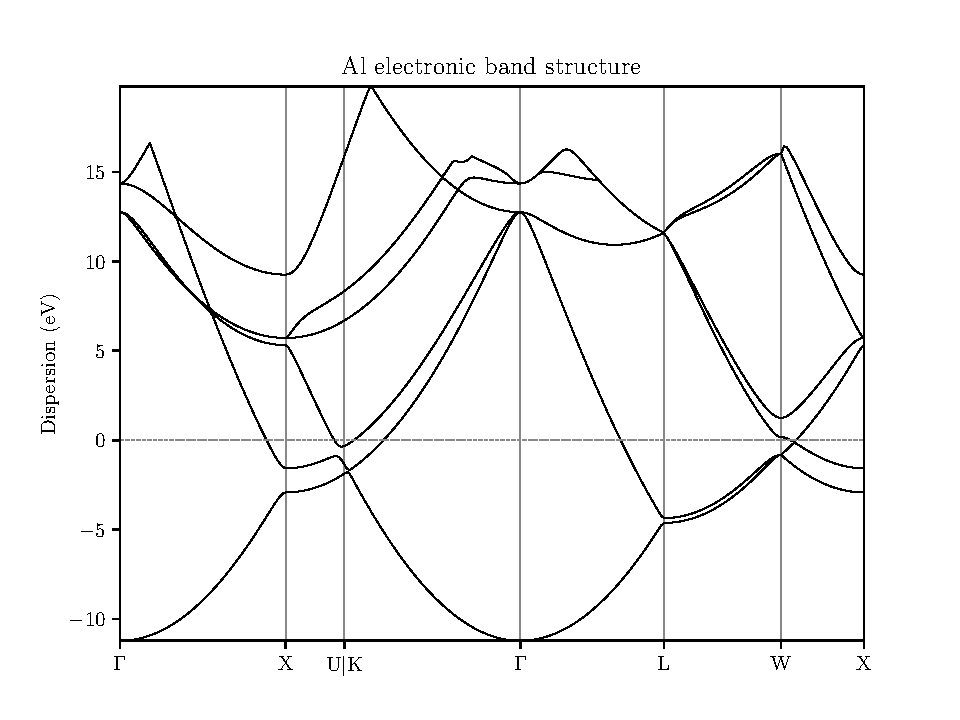
\includegraphics[width=.9\linewidth]{sections/images/bandstructures/Al_bands.pdf}
  \caption{Al}
  \label{fig:workchain_band_structures_Al}
\end{subfigure}%
\begin{subfigure}{.5\textwidth}
  \centering
  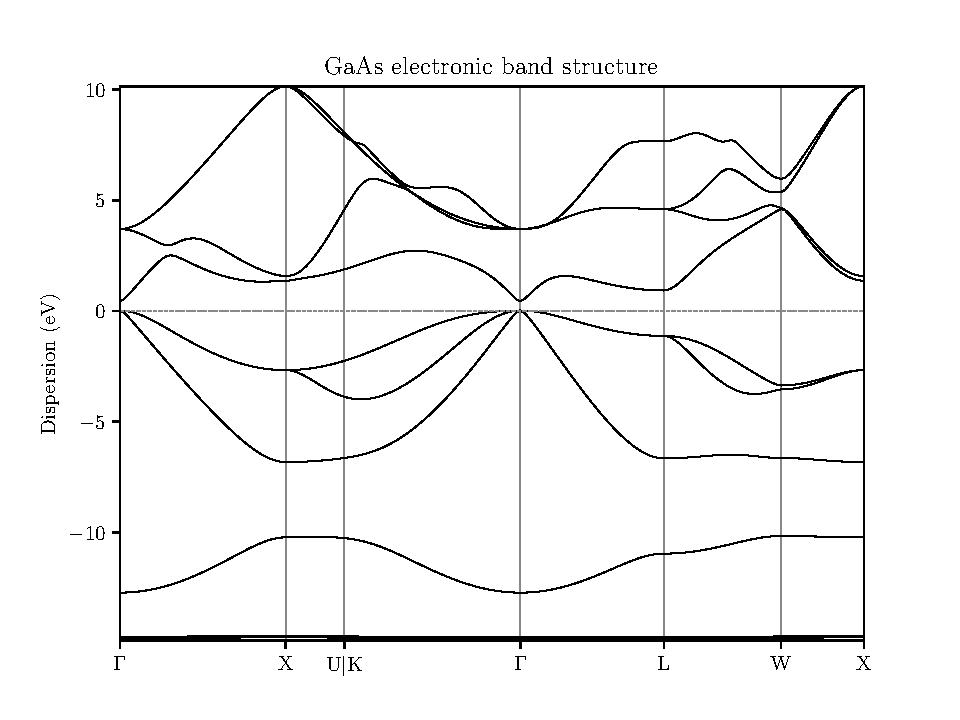
\includegraphics[width=.9\linewidth]{sections/images/bandstructures/GaAs_bands.pdf}
  \caption{GaAs}
  \label{fig:workchain_band_structures_GaAs}
\end{subfigure}%
\newline
\begin{subfigure}{.5\textwidth}
  \centering
  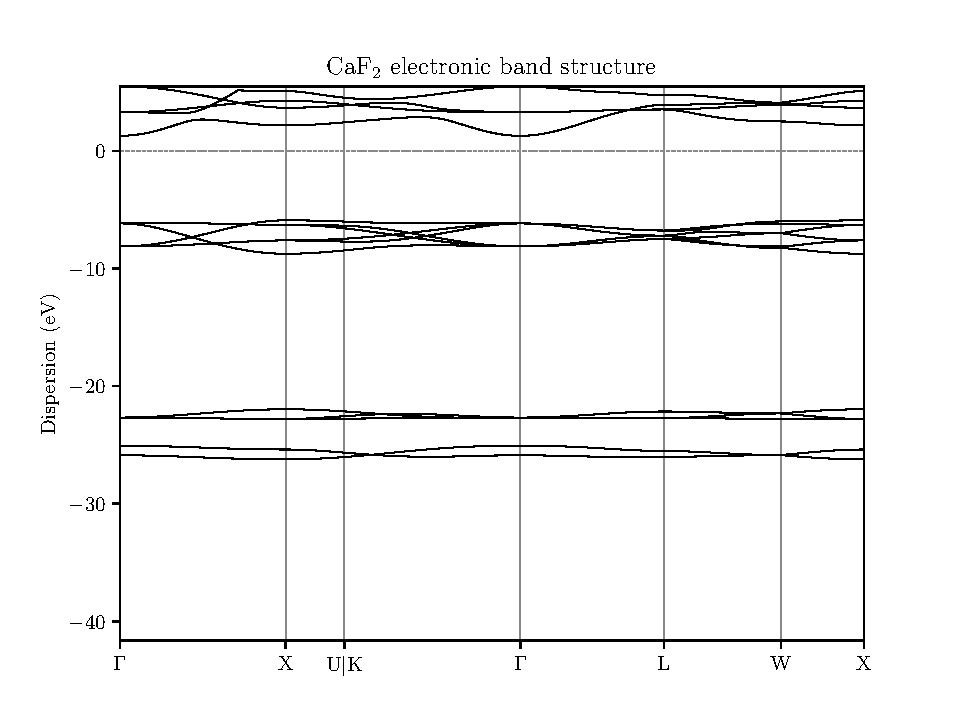
\includegraphics[width=.9\linewidth]{sections/images/bandstructures/CaF2_bands.pdf}
  \caption{CaF$_2$}
  \label{fig:workchain_band_structures_CaF2}
\end{subfigure}%
\begin{subfigure}{.5\textwidth}
  \centering
  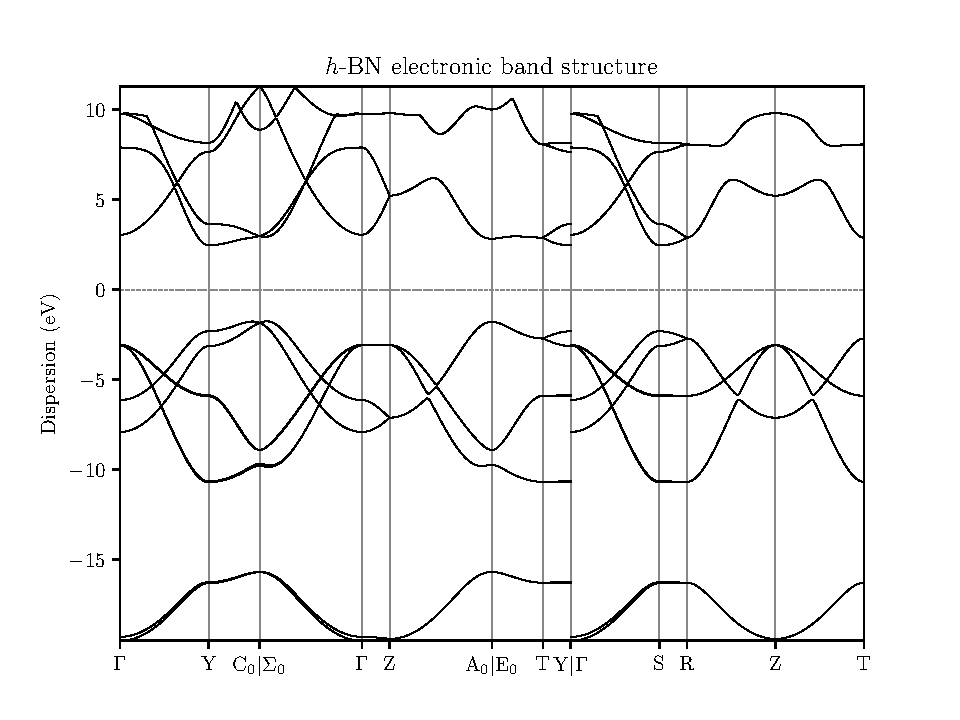
\includegraphics[width=.9\linewidth]{sections/images/bandstructures/hBN_bands.pdf}
  \caption{$h$-BN}
  \label{fig:workchain_band_structures_hBN}
\end{subfigure}%
\caption{Electronic band structures of four different crystal structures computed with AiiDA's PwBandsWorkChain}
\label{fig:workchain_band_structures}
\end{figure}


% Not included
%% !TEX root = ../AiiDA_tutorial_addition.tex
%%%%%%%%%%%
%Various Installation and setup procedures
%%%%%%%%%%%


\section[Installation and Setup]{Various installation and setup procedures}
\subsection{\label{sec:codesetup}Setting up a new computer and code in AiiDA: NWChem}

To be able to run a calculation, AiiDA needs to know certain information such as which computer the code can be found on and what the executable name is. In the main tutorial, for instance, you have been using an existing Quantum ESPRESSO pw code. 
You can check its name calling 
\begin{bashcommand}
verdi code list
\end{bashcommand}
and then inpsect its properties using
\begin{bashcommand}
verdi code show <CODENAME>
\end{bashcommand}

\begin{tcolorbox}
\textbf{Exercises:}
\begin{itemize}
\item
Setup a new code (for the simulation package NWChem)
\end{itemize}
\end{tcolorbox}

To learn how to setup a new code, let us configure AiiDA to be able to run NWChem, an open source computational chemistry package.  First we can check which calculation plugins are available:

\begin{bashcommand}
verdi calculation plugins
\end{bashcommand}

You will see an entry called \texttt{nwchem.pymatgen}.  This plugin creates the input and parses the output files and acts as the interface between AiiDA and NWChem (the parsing part is delegated to the pymatgen code, which explains the name of the plugin). To configure the code type:

\begin{bashcommand}
verdi code setup
\end{bashcommand}

Provide the following details to tell AiiDA about the code (if you want to learn more details on the \texttt{verdi code setup} command, refer to Appendix~\ref{app:codesetup} at page \pageref{app:codesetup}):

\begin{bashcommand}
=> Label: NWChem
=> Description: NWChem computational chemistry code
=> Local: False
=> Default input plugin: nwchem.pymatgen
=> Remote computer name: localhost
=> Remote absolute path: /usr/bin/nwchem
=> Text to prepend to each command execution
[Press CTRL+D for the next two steps]
\end{bashcommand}

If you want to inspect the details of the code you just generated, you can run
\begin{bashcommand}
verdi code show NWChem@localhost
\end{bashcommand}

\textbf{Note} Similarly, also new computers (e.g., a new cluster) can be configured using the \texttt{verdi computer setup} command, as we will see in Sec.~\ref{sec:computersetuptask}.

\subsubsection*{Task (optional, if you want to use the code you just created)}

\begin{tcolorbox}
\textbf{Exercise:}
\begin{itemize}
\item Run a simple simulation with the code NWChem
\end{itemize}
\end{tcolorbox}


Use the following \texttt{ParametersData} dict to run an NWChem calculation on silicon carbide:

\begin{pythoncommand}
parameters = ParameterData(dict={
    'directives': [
        ['set nwpw:minimizer', '2'],
        ['set nwpw:psi_nolattice', '.true.'],
        ['set includestress', '.true.']
    ],
    'geometry_options': [
        'units',
        'au',
        'center',
        'noautosym',
        'noautoz',
        'print'
    ],
    'memory_options': [],
    'symmetry_options': [],
    'tasks': [
        {
            'alternate_directives': {
                'driver': {'clear': '', 'maxiter': 40},
                'nwpw': {'ewald_ncut': 8, 
                         'simulation_cell': '\n  ngrid 16 16 16\n end'}
            },
            'basis_set': {},
            'basis_set_option': 'cartesian',            
            'charge': 0,
            'operation': 'optimize',
            'spin_multiplicity': None,
            'theory': 'pspw',
            'theory_directives': {},
            'title': None
        }
    ],
    'add_cell': True
})
\end{pythoncommand}

and we can use an ASE \texttt{Atoms} object to create the structure like so:

\begin{pythoncommand}
from ase import Atoms
asestruc = Atoms(['Si', 'Si', 'Si' ,'Si', 'C', 'C', 'C', 'C'],
    cell=[8.277, 8.277, 8.277])
asestruc.set_scaled_positions([
    (-0.5, -0.5, -0.5),
    (0.0, 0.0, -0.5),
    (0.0, -0.5, 0.0),
    (-0.5, 0.0, 0.0),
    (-0.25, -0.25, -0.25),
    (0.25 ,0.25 ,-0.25),
    (0.25, -0.25, 0.25),
    (-0.25 ,0.25 ,0.25),
])
structure = StructureData(ase=asestruc)
\end{pythoncommand}

The procedure is the same as before with QuantumEspresso except for fetching the NWCode.  This should take about a minute to run.

\begin{tcolorbox}
\textbf{Exercise:}
\begin{itemize}
\item Inspect the results.
\end{itemize}
\end{tcolorbox}

Once the calculation is done you can retrieve the calculation node using the PK from \texttt{verdi calculation list -a -p1}.  After loading the node have a look at \texttt{node.out.trajectory}.  This stores information about the positions of the atoms at each relaxation steps.  You can for instance see how the cell evolved by printing
\cmd{node.out.trajectory.get\_cells()}, and how the positions changed with 
\cmd{node.out.trajectory.get\_positions()}.


\section{\label{sec:computersetuptask}Setup a new computer}
\subsection{Setting up the computer in the database}
Until now, we just had on computer configured in the test machine, called \texttt{localhost}. To see all computers configured, you can use
\begin{bashcommand}
verdi computer list
\end{bashcommand}

\begin{tcolorbox}
\textbf{Exercise:}
\begin{itemize}
\item Install a new computer (the test machine of your neighbor).
\item Check if the installation was successful.
\end{itemize}
\end{tcolorbox}

\subsubsection*{Preliminary steps}
\begin{itemize}
\item As a first step, choose a computer you have. You can try to setup this machine.
If you don't have one, or you want to try a tested setup, you can setup the same computer on which
you are running the tests, but this time not with a local transport, but via SSH, as an example. The instructions below are for this use case. We will call the computer \texttt{localhost-ssh}.

\item Generate a new ssh key pair, without passphrase:
\begin{verbatim}
    ssh-keygen
\end{verbatim}
and press enter when asked. 
Copy the content of the \texttt{$\sim$/.ssh/id\_rsa.pub} file that was created and 
paste it as a new line into the file \texttt{$\sim$/.ssh/authorized\_keys}. \textbf{IMPORTANT!}
Append it to the file, without modifying the current content, otherwise you will 
not be able to ssh into the machine again.

\item Check that you can connect to the computer: from the shell, run \texttt{ssh localhost} and check that you can connect. Then, logout (only once to close the ssh session;
you should remain on the tutorial machine).
\end{itemize}

Now you are ready to setup the computer.

\begin{tcolorbox}
\textbf{Exercise:}
\begin{itemize}
\item Run the command \texttt{verdi computer setup} to install the computer called \texttt{localhost-ssh}. See below for some hints.
\end{itemize}
\end{tcolorbox}

Hints:
\begin{itemize}
\item Read appendix~\ref{app:computersetup} for an explanation of the various items you will be asked for
\item Type \texttt{localhost} when you are asked for the fully-qualified hostname
\item As transport, use SSH; as scheduler, write \texttt{torque}
\item As work directory, you can use \texttt{/home/\{username\}/.aiida\_run}
\item As MPI run command, the default value should be OK: \texttt{mpirun -np \{tot\_num\_mpiprocs\}}
\item set only 2 CPU per machine for this tutorial
\item Leave empty the next two prepend/append strings (you need to press CTRL+D as indicated)
\end{itemize}

\subsection{Configuring the computer connection credentials}

You can now type \texttt{verdi computer list -a} to see that you computer is now present (\texttt{-a} to show all computers, also the unconfigured ones and the ones not setup by you). 

You will notice that your computer is marked as ``unconfigured'' (and you might see also other unconfigured computers, coming with the import data that we used in earlier parts of this tutorial). Indeed, the command \cmd{verdi computer setup} just creates a reference for the computer in your database. Something similar also happens when you import data. However, if you want to run simulations with a computer, you need also to specify the credentials of how to connect to it. 

To do this, you need to run 
\begin{bashcommand}
verdi computer configure COMPUTERNAME
\end{bashcommand}

\begin{tcolorbox}
\textbf{Exercise:}
\begin{itemize}
\item Configure your computer with the above command (see hints below)
\item Check if AiiDA can connect to the computer
\end{itemize}
\end{tcolorbox}

Hints:
\begin{itemize}
\item If you properly set up the \texttt{$\sim$/.ssh/config} file in the step before, AiiDA will read that information and all parameters will be already set by default. You just need to press Enter. 
\item Still, try to understand each item---you can refer to Appendix~\ref{sec:computerconfigure} for a detailed explanation of each item.
\end{itemize}

When you are done, you can test if everything worked by running
\begin{bashcommand}
verdi computer test COMPUTERNAME
\end{bashcommand}
If everything worked, The last line should read something like ``Test completed (all tests succeeded)''.

\subsection{Final useful commands}
To get information on a specific computer, run:
\begin{bashcommand}
verdi computer show COMPUTERNAME
\end{bashcommand}

It is also possible to enable/disable a computer with the command
\begin{bashcommand}
verdi computer enable COMPUTERNAME
verdi computer disable COMPUTERNAME
\end{bashcommand}
The last two commands might be useful when new resources might
or not be available (e.g. during maintenance), 
so that you can still submit calculations to
AiiDA, but AiiDA will not try to connect to the computer until when
you enable the computer again.

\begin{tcolorbox}
\textbf{Exercise (optional):}
\begin{itemize}
\item Configure the Quantum ESPRESSO code as explained in Sec.~\ref{sec:codesetup}. 
To know the \texttt{pw.x} executable path, that you will need during the 
code configuration, you can find it in the output of \texttt{verdi code show CODENAME} for the code that was already setup for you and that you used during the tutorial (on the machine \texttt{localhost} that uses a \texttt{local} transport -- you are instead
setting up the same code but on the \texttt{localhost-ssh} machine, that uses a \texttt{ssh} transport).
\item Try to run a simulation with this code, to see if it works, as explained in the main tutorial.
\end{itemize}
\end{tcolorbox}





\begin{appendices}
\section{\label{app:computersetup}Options when setting up and configuring a computer}
\subsection{\texttt{verdi computer setup}} 
Here is a list of what is asked during the execution of \cmd{verdi computer setup}, together with an explanation of each item.

\begin{itemize}

\item {} 
\textbf{Computer name}: the (user-friendly) name of the new computer instance
which is about to be created in the DB (the name is used for instance when
you have to pick up a computer to launch a calculation on it). Names must
be unique. This command should be thought as a AiiDA-wise configuration of
computer, independent of the AiiDA user that will actually use it.

\item {} 
\textbf{Fully-qualified hostname}: the fully-qualified hostname of the computer
to which you want to connect. 

\item {} 
\textbf{Description}:  A human-readable description of this computer; this is
useful if you have a lot of computers and you want to add some text to
distinguish them (e.g.: ``cluster of computers at EPFL, with 434 nodes, 2 GB of RAM per CPU'')

\item {} 
\textbf{Enabled}: either True or False; if False, the computer is disabled
and calculations associated with it will not be submitted. This allows to
disable temporarily a computer if it is giving problems or it is down for
maintenance, without the need to delete it from the DB.

\item {} 
\textbf{Transport type}: The name of the transport to be used. A list of valid
transport types can be obtained typing \textit{?}

\item {} 
\textbf{Scheduler type}: The name of the plugin to be used to manage the
job scheduler on the computer. A list of valid
scheduler plugins can be obtained typing \textit{?}.

\item {}
\textbf{shebang line at the beginning of the submission script}: 
The first line of any submission script. The default is \texttt{\#!/bin/bash}.
This is often used by the scheduler to decide which shell to use. AiiDA expects
this to be bash, but some supercomputer need a login shell, and then you need
to specify \texttt{\#!/bin/bash -l}.

\item {} 
\textbf{AiiDA work directory}: The absolute path of the directory on the
remote computer where AiiDA will run the calculations
(often, it is the scratch of the computer). You can (should) use the
\textit{\{username\}} replacement, that will be replaced by your username on the
remote computer automatically: this allows the same computer to be used
by different users, without the need to setup a different computer for
each one.

\item {} 
\textbf{mpirun command}: The \cmd{mpirun} command needed on the cluster to run parallel MPI
programs. You can (should) use the \textit{\{tot\_num\_mpiprocs\}} replacement,
that will be replaced by the total number of cpus, or the other
scheduler-dependent fields. 

\item {}
\textbf{Default number of CPUs}: Setup the number of CPUs per node of the cluster. In this way, if you specify to use one node (a 'machine' in AiiDA), the calculation will try by default to use all the CPUs of the node.

\item {} 
\textbf{Text to prepend to each command execution}: This is a multiline string,
whose content will be prepended inside the submission script before the
real execution of the job. It is your responsibility to write proper \cmd{bash} code!
This is intended for computer-dependent code, like for instance loading a
module that should always be loaded on that specific computer. \emph{Remember}
\emph{to end the input by pressing} \textit{\textless{}CTRL\textgreater{}+D}.

\item {} 
\textbf{Text to append to each command execution}: This is a multiline string,
whose content will be appended inside the submission script after the
real execution of the job. It is your responsibility to write proper \cmd{bash} code!
This is intended for computer-dependent code. \emph{Remember}
\emph{to end the input by pressing} \textit{\textless{}CTRL\textgreater{}+D}.

\end{itemize}

\subsection{\label{sec:computerconfigure}\texttt{verdi computer configure}}
To setup the credentials to be able to run on a computer, you should use the following command:
\begin{bashcommand}
verdi computer configure COMPUTERNAME
\end{bashcommand}

When using the SSH transport, the command will try to provide automatically default answers, mainly reading
the existing ssh configuration in \textbf{\textasciitilde{}/.ssh/config}, and in most cases one
simply need to press enter a few times.

At the moment, the in-line help (i.e., just typing \textbf{?} to get
some help) is not yet supported in \cmd{verdi configure}, but only in
\cmd{verdi setup}.

The following options will be asked for ssh transport type.

\begin{itemize}
\item {} 
\textbf{username}: your username on the remote machine

\item {} 
\textbf{port}: the port to connect to (the default SSH port is 22)

\item {} 
\textbf{look\_for\_keys}: automatically look for the private key in \textbf{\textasciitilde{}/.ssh}.
Default: True.

\item {} 
\textbf{key\_filename}: the absolute path to your private SSH key. You can leave
it empty to use the default SSH key, if you set \textbf{look\_for\_keys} to True.

\item {} 
\textbf{timeout}: A timeout in seconds if there is no response (e.g., the
machine is down). You can leave it empty to use the default value.

\item {} 
\textbf{allow\_agent}: If True, it will try to use an SSH agent.

\item {} 
\textbf{proxy\_command}: Leave empty if you do not need a proxy command (i.e.,
if you can directly connect to the machine).

\item {} 
\textbf{compress}: True to compress the traffic (recommended)

\item {} 
\textbf{gss\_auth, gss\_kex, gss\_deleg\_creds, gss\_host}: These are parameters needed if your cluster requires authentication via Kerberos. If you don't know what Kerberos is, just ignore these four variables and leave their value to the default one (in particular, \texttt{gss\_auth = no}). Otherwise, read the documentation of AiiDA (and of the paramiko python package) online for more details.

\item {} 
\textbf{load\_system\_host\_keys}: True to load the known hosts keys from the
default SSH location (recommended)

\item {} 
\textbf{key\_policy}: What is the policy in case the host is not known.
It is a string among the following:
\begin{itemize}
\item {} 
\textbf{RejectPolicy} (default, recommended): reject the connection if the
host is not known.

\item {} 
\textbf{WarningPolicy} (\emph{not} recommended): issue a warning if the
host is not known.

\item {} 
\textbf{AutoAddPolicy} (\emph{not} recommended): automatically add the host key
at the first connection to the host.

\end{itemize}

\end{itemize}

\section{\label{app:codesetup}Setting up a code: \texttt{verdi code setup} options}

Once you have at least one computer configured, you can configure the codes, using the command \cmd{verdi code setup}.

In AiiDA, for full reproducibility of each calculation, we store each code in the database, and attach to each calculation a given code. This has the further advantage to make it very easy to query for all calculations that were run with a given code (for instance because I am looking for phonon calculations, or because I discovered that a specific version had a bug and I want to rerun the calculations).

In AiiDA there are two types of codes:

\begin{itemize}
 \item \textbf{Remote codes} are installed on a remote computer like a supercomputer.
 \item \textbf{Local codes} are not already present on the remote machine and must be copied for every submission. 
\end{itemize}

The command \cmd{verdi code setup} will ask several values. Here is a description of their meaning.

\begin{itemize}
\item {} 
\textbf{label}:  A label to refer to this code. Note: this label is not enforced
to be unique. However, if you try to keep it unique, you can use it later
to refer and use to your code. Otherwise, you need to remember its ID or UUID.

\item {} 
\textbf{description}: A human-readable description of this code (for instance ``Quantum
Espresso v.5.0.2 with 5.0.3 patches, pw.x code, compiled with openmpi'')

\item {} 
\textbf{default input plugin}: A string that identifies the default input plugin to
used to generate new calculations to use with this code.
This string has to be a valid string recognised by the \textbf{CalculationFactory}
function. To get the list of all available Calculation plugin strings,
use the \cmd{verdi calculation plugins} command. Note: if you do not want to
specify a default input plugin, you can write the string ``None'', but this is
discouraged, because then you will not be able to use
the \textbf{.get\_builder()} method of the \textbf{Code} object.

\item {} 
\textbf{local}: either True (for local codes) or False (for remote
codes). For the meaning of the distinction, see above. Depending
on your choice, you will be asked for:
\begin{itemize}
\item {} 
LOCAL CODES:
\begin{itemize}
\item {} 
\textbf{Folder with the code}: The folder on your local computer in which there
are the files to be stored in the AiiDA repository, and that will then be
copied over to the remote computers for every submitted calculation.
This must be an absolute path on your computer.

\item {} 
\textbf{Relative path of the executable}: The relative path of the executable
file inside the folder entered in the previous step.

\end{itemize}

\item {} 
REMOTE CODES:
\begin{itemize}
\item {} 
\textbf{Remote computer name}: The computer name as on which the code resides,
as configured and stored in the AiiDA database

\item {} 
\textbf{Remote absolute path}: The (full) absolute path of the code executable
on the remote machine

\end{itemize}

\end{itemize}

\end{itemize}
\end{appendices}


\begin{appendices}
\phantomsection
\addcontentsline{toc}{part}{Appendices}\part*{Appendices}
\emph{The following appendices consist of optional exercises, and are mentioned in earlier parts of the tutorial. Go through them only if you have time.}
% !TEX root = ../AiiDA_tutorial.tex
\section{Calculation input validation}
This appendix shows additional ways to debug possible errors with QE, how to use a useful tool that we included in AiiDA to validate the input to Quantum ESPRESSO (and possibly suggest the correct name to mispelled keywords)

There are various reasons why you might end up providing a wrong input to a Quantum ESPRESSO calculation.
Let's check for example this input dictionary, where we inserted two mistakes:
\begin{pythoncommand}
parameters_dict = {
    "CTRL": {
        "calculation": "scf",
        "restart_mode": "from_scratch",
    },
    "SYSTEM": {
        "nat": 2,
        "ecutwfc": 30.,
        "ecutrho": 200.,
    },
    "ELECTRONS": {
        "conv_thr": 1.e-6,
    }
}
\end{pythoncommand}

The two mistakes in the dictionary are the following.
First, we wrote a wrong namelist name ('CTRL' instead of 'CONTROL').
Second, we inserted the number of atoms explicitly: while that is how the number of atoms is specified in Quantum ESPRESSO, in AiiDA this key is reserved by the system: in fact this information is already contained in the StructureData. Modify the script with this ParameterData. 
In this case, we use a tool (the input validator that we provide in AiiDA) to check the input file before submitting. Therefore, the behavior will be slightly different from the previous example: the plugin will check for some keys and will refuse to submit the calculation.
This kind of mistakes is revealed by either
\begin{itemize}
\item Submitting a calculation. You will see the calculation ending up in the SUBMISSIONFAILED status. Check therefore the logs to recognize the source of the error.
\item Submitting a test. You will not be able to successfully create the test and the traceback will guide you to the problem.
\end{itemize}


Over the time this kind of trivial mistakes can be annoying, but they can be avoided with a utility function that checks the ``grammar'' of the input parameters.
In your script, after you defined the parameters\_dict, you can validate it with the command
(note that you need to pass also the input crystal structure, \texttt{s}, to
allow the validator to perform all needed checks):

\begin{pythoncommand}
PwCalculation = CalculationFactory('quantumespresso.pw')
validated_dict = PwCalculation.input_helper(parameters_dict, structure=s)
parameters = ParameterData(dict=validated_dict)
\end{pythoncommand}

The \texttt{input\_helper} method will check for the correctness of the input parameters.
If misspelling or incorrect keys are detected, the method raises an exception, which stops the script before submitting the calculation and thus allows for a more effective debugging.

With this utility, you can also provide a list of keys, without providing the namelists (useful if you don't remember where to put some variables in the input file).
Hence, you can provide to \texttt{input\_helper()} a dictionary like this one:
\begin{pythoncommand}
parameters_dict = {
    'calculation': 'scf',
    'tstress': True,
    'tprnfor': True,
    'ecutwfc': 30.,
    'ecutrho': 200.,
    'conv_thr': 1.e-6,
}
validated_dict = PwCalculation.input_helper(
    parameters_dict, structure=s, flat_mode=True)
\end{pythoncommand}
If you print the \texttt{validated\_dict}, it will look like:
\begin{pythoncommand}
{
    "CONTROL": {
        "calculation": "scf",
        "tstress": True,
        "tprnfor": True,
    },
    "SYSTEM": {
        "ecutwfc": 30.,
        "ecutrho": 200.,
    },
    "ELECTRONS": {
        "conv_thr": 1.e-6,
    }
 }
\end{pythoncommand}



\section{Restarting calculations}
Up to now, we have only presented cases in which we were passing wrong input parameters to the calculations, which required us to modify the input scripts and relaunch calculations from scratch.
There are several other scenarios in which, more generally, we need to restart calculations from the last step that they have executed.
For example when we run molecular dynamics, we might want to add more time steps than we initially thought, or as another example you might want to refine the relaxation of a structure with tighter parameters.

In this section, you will learn how to restart and/or modify a calculation that has run previously. As an example, let us first submit a total energy calculation using a parameters dictionary of the form:
\begin{pythoncommand}
parameters_dict = {
    'CONTROL': {
        'calculation': 'scf',
        'tstress': True,
        'tprnfor': True,
    },
    'SYSTEM': {
        'ecutwfc': 30.,
        'ecutrho': 200.,
    },
    'ELECTRONS': {
        'conv_thr': 1.e-14,
        'electron_maxstep': 3,
    },
}
\end{pythoncommand}
and submit the calculation with this input.
In this case, we set a very low number of self consistent iterations (3), too small to be able to reach the desired accuracy of 10$^{-14}$: therefore the calculation will not reach a complete end and will be flagged in a FAILED state. However, there is no mistake in the parameter dictionary.

Now, create a new script file, where you will try to restart and correct the input dictionary.
We first load the calculation that has just failed (let's call it \texttt{c1})
\begin{pythoncommand}
old_calc = load_node(PK)
\end{pythoncommand}
(take care of using the correct PK).
Then, create a new Builder \texttt{builder} which is set to reuse all inputs
from the previous step, with a few adaptations to the input parameters
that might be needed by the code to properly deal with restarts. 
\begin{pythoncommand}
from aiida_quantumespresso.utils.restart import create_restart_pw
builder = create_restart_pw(                                     
   old_calc,                            
   use_output_structure=False,  
   restart_from_beginning=False, 
   force_restart=True)
\end{pythoncommand}
The flag usage (most of them are optional) is:
\begin{itemize}
 \item \texttt{use\_output\_structure}: if True and \texttt{old\_calc} has an output structure, the new calculation will use it as input; 
 \item \texttt{restart\_from\_beginning}: if False the new calculation will start from the charge density of \texttt{old\_calc}, it will start from the beginning otherwise;
 \item \texttt{force\_restart}: if True, the new calculation will be created even 
 if \texttt{old\_calc} is not in a FINISHED job state.
\end{itemize}

Since this calculation has exactly the same parameters of before, we have to modify the input parameters and increase \texttt{electron\_maxstep} to a larger value.
To this aim, let's load the dictionary of values and change it
\begin{pythoncommand}
old_parameters = builder.parameters
parameters_dict = old_parameters.get_dict()
parameters_dict['ELECTRONS']['electron_maxstep'] = 100
\end{pythoncommand}
Note that you cannot modify the \texttt{old\_parameters} object: it has been used by calculation \texttt{c1} and is saved in the database; hence a modification would break the provenance.
We have to create a new ParameterData and pass it to c2:
\begin{pythoncommand}
ParameterData = DataFactory('parameter')
new_parameters = ParameterData(dict=parameters_dict)
builder.parameters = new_parameters
\end{pythoncommand}
Now you can launch the new calculation
\begin{pythoncommand}
from aiida.work.run import submit    
new_calc = submit(builder)
print new_calc.pk
\end{pythoncommand}
that this time can proceed until the end and return converged total energy.
Using the restart method, the script is much shorter than the one needed to launch a new one from scratch: you didn't need to define pseudopotentials, structures and k-points, which are the same as before. 
You can indeed inspect the new calculation to check that now it actually 
completed successfully.
% !TEX root = ../AiiDA_tutorial.tex
\section{Queries in AiiDA - Optional examples and exercises}


\subsection*{Optional exercises on relationships (Task 3)}
\textbf{Hint for the exercises:}
\begin{itemize}
\item You can have projections on properties of more than one entity in your query. You just have to add the \emph{project} key (specifying the list of properties that you want to project) along with the corresponding entity when you append it.
\end{itemize}

\begin{tcolorbox}
\textbf{Exercises:}\\~\\
Try to write the following queries:
\begin{itemize}
	\item Find all descendants of a StructureData with a certain uuid. Print both the StructureData and the descendant.
	\item Find all the FolderData created by a specific user.
\end{itemize}
\end{tcolorbox}

\subsection*{Optional exercises on attributes and extras (Task 4)}
\textbf{Hint for the exercises:}
\begin{itemize}
\item You can easily order or limit the number of the results by using the \emph{order\_by()} and \emph{limit()} methods of the QueryBuilder. For example, we can order all our job calculation by their \textit{id} and limit the result to the first 10 as follows:
\begin{pythoncommand}
qb = QueryBuilder()
qb.append(JobCalculation, tag='calc')
qb.order_by({'calc':'id'})
qb.limit(10)
qb.all()
\end{pythoncommand}
\end{itemize}

\begin{tcolorbox}
\textbf{Exercises:}
\begin{itemize}
    \item Write a code snippet that informs you how many pseudopotentials you have for each element.
    \item Smearing contribution to the total energy for calculations:
    \begin{enumerate}
        \item Write a query that returns the smearing contribution to the energy stored in some instances of ParameterData.
        \item Extend the previous query to also get the input structures.
        \item Which structures have a smearing contribution to the energy smaller or equal to -0.02?
    \end{enumerate}
\end{itemize}
\end{tcolorbox}

\subsection*{Summarizing what we learned by now - An example}
At this point you should be able to do queries with projections, joins and filters. Moreover, you saw how to apply filters and projections even on attributes and extras. Let's discover the full power of the QueryBuilder with a complex graph query that allows you to project various properties from different nodes and apply different filters and joins.

Imagine that you would like to get the smearing energy for all the calculations that have finished and have a $\mathrm{Sn_{2}O_{3}}$ as input. Moreover, besides from the smearing energy, you would like to print the units of this energy and the formula of the structure that was given to the calculation.
The graphical representation of this query can be seen in Figure~\ref{fig:qb2} and the actual query follows:
\begin{figure}[!th]
\begin{center}
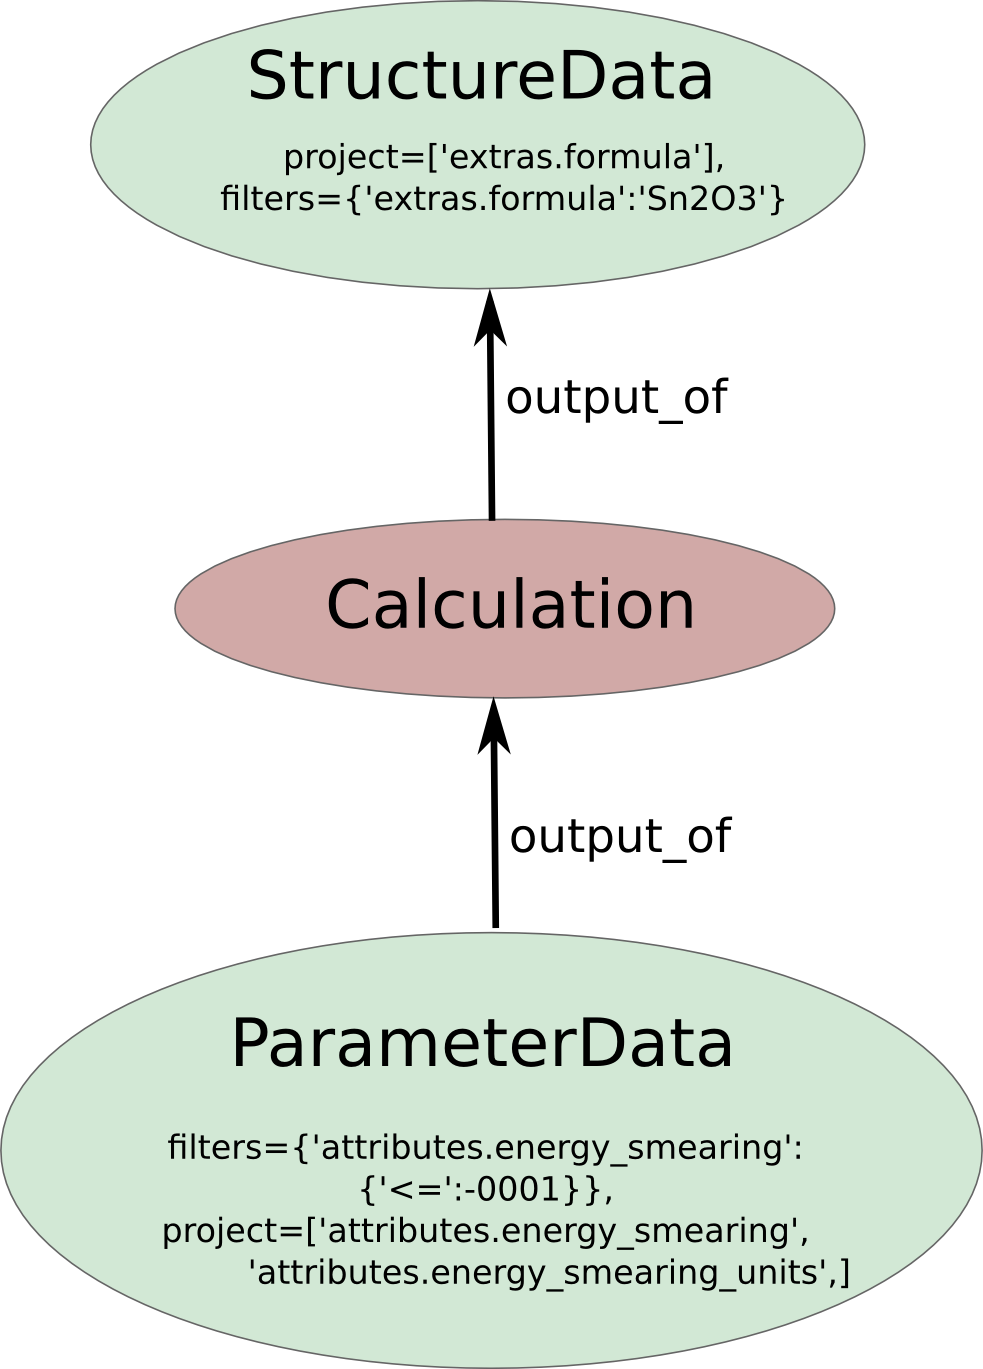
\includegraphics[width=7cm]{img/qb_example_2.png}
\end{center}
\caption{Complex graph query.}
\label{fig:qb2}
\end{figure}

\begin{pythoncommand}
qb = QueryBuilder()
qb.append(
        StructureData,
        project=["extras.formula"],
        filters={"extras.formula":"Sn2O3"},
        tag="structure"
    )
qb.append(
        Calculation,
        tag="calculation",
        output_of="structure"
    )
qb.append(
        ParameterData,
        tag="results",
        filters={"attributes.energy_smearing":{"<=":-0.0001}},
        project=[
            "attributes.energy_smearing",
            "attributes.energy_smearing_units",
        ],
        output_of="calculation"
)
qb.all()
\end{pythoncommand}

\section{\label{sec:convpressure}More complex logic in workflows: while loops and conditional statements}
In the previous sections, you have been introduced to WorkChains, and the reason for using them over ``standard'' workfunctions (i.e., functions decorated with \cmd{@wf}).

However, in the example of Sec.~\ref{sec:workchainsimple}, the \cmd{spec.outline} was quite simple, with a ``static'' sequence of two steps.
Most often, however, you need dynamic workflows, where you need to decide at runtime whether to continue to compute or not (e.g. in a convergence loop, where you need to stop if convergence has been achieved).
To support this scenario, the \cmd{spec.outline} can support logic: \emph{while} loops and \emph{if/elif/else} blocks.
The simplest way to explain it is to show an example:
\begin{pythoncommand}
from aiida.work.workchain import if_, while_

spec.outline(
    cls.s1,
    if_(cls.isA)(
        cls.s2
    ).elif_(cls.isB)(
        cls.s3
    ).else_(
        cls.s4
    ),
    cls.s5,
    while_(cls.condition)(
        cls.s6
    ),
)
\end{pythoncommand}
that would \emph{roughly} correspond, in a python syntax, to:
\begin{pythoncommand}
s1()
if isA():
    s2()
elif isB():
    s3()
else:
    s4()
s5()
while condition():
    s6()
\end{pythoncommand}
The only constraint is that condition functions (in the example above \cmd{isA}, \cmd{isB} and \cmd{condition}) must be class methods that returns \texttt{True} or \texttt{False} depending on whether the condition is met or not.

A suggestion on how to write new workchains: Use the outline to help you in designing the logic. First create the spec outline writing, almost if you were explaining it in words, what you expect the workflow to do. Then, define one by one the methods.
For example, we have prepared a simple workfunction to optimize the lattice parameter of silicon efficiently using a Newton's algorithm on the energy derivative, i.e. the pressure $p=-dE/dV$. You can find it the code at \texttt{tutorial\_scripts/pressure\_convergence.py}. 
The outline looks like this:
\begin{pythoncommand}
spec.outline(
    cls.init,
    cls.put_step0_in_ctx,
    cls.move_next_step,
    while_(cls.not_converged)(
        cls.move_next_step,
     ),
    cls.report
)
\end{pythoncommand}
This outline already roughly explains the algorithm: after an initialization (\cmd{init}) and putting the first step (number zero) in the ctx (\cmd{put\_step0\_in\_ctx}), a function to move to the next step is called (\cmd{move\_next\_step}). This is iterated while a given convergence criterion is not met (\cmd{not\_converged}). Finally, some reporting is done, including returning some output nodes (\cmd{report}).

If you are interested in the details of the algorithm, you can inspect the file. The main ideas are described here:
\begin{description}
\item[init] Generate a \texttt{pw.x} calculation for the input structure (with volume $V$), and one for a structure where the volume is $V+4\text{\AA}^3$ (just to get a closeby volume). Store the results in the context as \cmd{r0} and \cmd{r1}
\item[put\_step0\_in\_ctx] Store in the context $V$, $E(V)$ and $dE/dV$ for the first calculation \cmd{r0}
\item[move\_next\_step] This is the most important function. Calculate $V$, $E(V)$ and $dE/dV$ for \cmd{r1}. Also, estimate $d^2E/dV^2$ from the finite difference of the first derivative of \cmd{r0} and \cmd{r1} (helper functions to achieve this are provided).
Get the $a$, $b$ and $c$ coefficients of a parabolic fit $E=aV^2 + bV + c$ and estimated the expected minimum of the EOS function as the minimum of the fit $V_0=-b/2a$. Finally, replace \cmd{r0} with \cmd{r1} in the context (i.e., get rid of the oldest point) and launch a new pw calculation at volume $V_0$, that will be stored in the context replacing \cmd{r1}. In this way, at the next iteration \cmd{r0} and \cmd{r1} will contain the latest two simulations. Finally, at each step some relevant information (coefficients $a$, $b$ and $c$, volumes, energies, energy derivatives, ...) are stored in a list called \cmd{steps}. This whole list is stored in the context because it provides quantities to be preserved between different workfunction steps.
\item[not\_converged] Return \cmd{True} if convergence has not been achieved yet. Convergence is achieved if the difference in volume between the two latest simulations is smaller than a given threshold (\cmd{volume\_tolerance}).
\item[report] This is the final step. Mainly, we return the output nodes: \cmd{steps} with the list of results at each step, and \cmd{structure} with the final converged structure.
\end{description}

The results returned in \cmd{steps} can be used to represent the evolution of the minimisation algorithm. A possible way to visualize it is presented in Fig.~\ref{fig:convpressure}, obtained with an initial lattice constant of $a_{\text{lat}} = 5.2\text{\AA}$. 
%You can try to reproduce the same graph by running the WorkChain and then using the script \texttt{tutorial\_scripts/plot\_convergence\_pressure.py} to generate the same plot.

\begin{figure}[tb]
\centering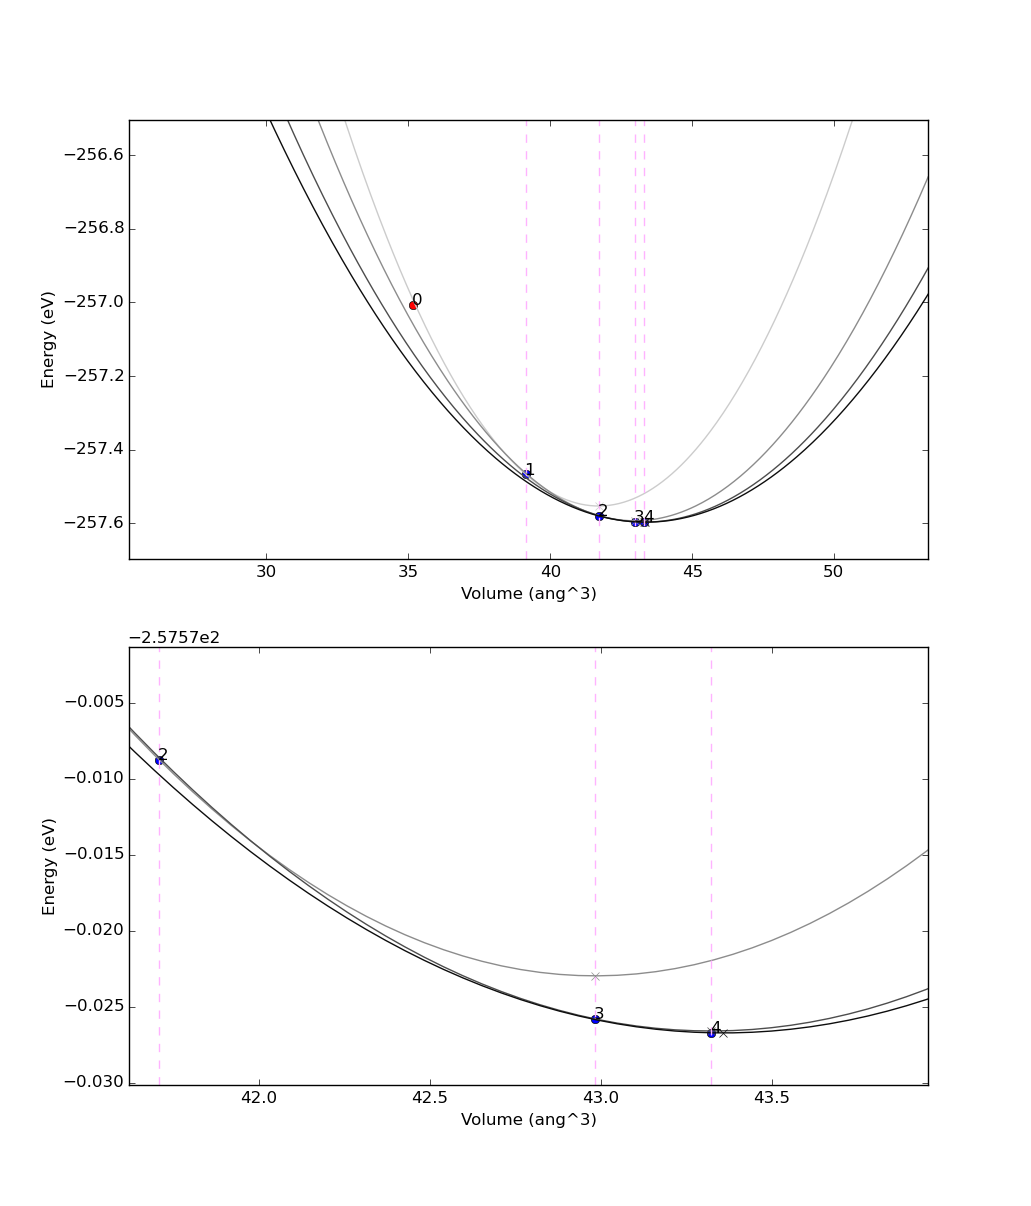
\includegraphics[width=0.6\linewidth]{img/convergence_pressure}
\caption{\label{fig:convpressure}Example of results of the convergence algorithm presented in Sec.~\ref{sec:convpressure}. The bottom plot is a zoom near the minimum. The dots represent the (volume,energy) points obtained from Quantum ESPRESSO, and the numbers indicate at which iteration they were obtained. The parabolas represent the parabolic fits used in the algorithm; the minimum of the parabola is represented with a small cross, in correspondence of the vertical lines, used as the volume for the following step.}
\end{figure} 



\end{appendices}

